\documentclass{article}
\usepackage{amsmath,amssymb, amsfonts}
\usepackage{algorithm}
\usepackage{float}
\usepackage{subcaption}
 \usepackage{relsize}
\usepackage{graphicx}
\usepackage{booktabs} 
\usepackage[table]{xcolor}
\usepackage{bm}
\usepackage{setspace}
\usepackage{amsthm}
\usepackage{graphicx}
\usepackage{algorithm}
\usepackage{algpseudocode}
\usepackage{cite}
\usepackage{geometry}
 \geometry{
 letterpaper,
 total={8.5in,11in},
 left=1.25in,
 right=1in,
 top=1in,
 bottom=1in,
 }
\doublespace
\newcolumntype{\Ca}{$Ca^{2+}$}
\newcommand{\commJoey}[1]{{\color{red}{\em Joey: #1}}}
\newcommand{\commTim}[1]{{\color{blue}{\em Tim: #1}}}
\newcommand{\commPierre}[1]{{\color{green}{\em Pierre: #1}}}

\def\r{{\mathbb R}}

\begin{document}
All of the work described below uses the model Tim emailed to Joey on October 13, 2017; the codes are included in OO-NVU-20.zip saved in the repository. Our objective is to identify which parameters in the model govern the dynamics of the potassium, the state $K_e$ in the model, during the period when a current is applied.

As a first step we allowed 70 parameters to vary on a uniform interval about their nominal value with 10\% uncertainty. These 70 parameters are found in the following channels within the ``Neuron.m" file contained in OO-NVU-20.zip,
\begin{enumerate}
\item[$\bullet$] Na flux through NaP channel in soma using GHK
\item[$\bullet$] Na flux through NaT channel in soma using GHK
\item[$\bullet$] K flux through KDR channel in soma using GHK
\item[$\bullet$] K flux through KA channel in soma using GHKinput\_current
\item[$\bullet$] Na flux through NaP channel in dendrite using GHK
\item[$\bullet$] Na/K flux through NMDA channel in dendrite using GHK
\item[$\bullet$] K flux through KDR channel in dendrite using GHK
\item[$\bullet$] K flux through KA channel in dendrite using GHK
\end{enumerate}

We generated 1000 realizations of these parameters (assuming them to be independent) and solved the ODE system for each realization. Of these 1000 realizations, 167 of them did not return a solution for the entire time interval; we expect that the ODE solver was unable to solve for those parameter values. There were also 3 realizations where the ODE solver returned complex solutions, these where discarded as well. This left 830 realizations to be used for the subsequent analysis.

Using the 830 realizations we are able to identify that around 24 of them yielded a potassium profile consistent with experimental data. This seems to indicate that there exists a subset of the parameters under consideration which give the desired dynamics. Upon inspection of histograms and correlation plots, we hypothesize that to understand the parameters yielding results comparable to experimental data we must understand the correlation structure of the parameters. We assumed them to be independent because we have no further knowledge at this time. If we can solve a Bayesian inverse problem we may discovered the desired correlation structure, but this is too computationally intensive with the current parameter dimension and model complexity. 

Using the 830 realizations we constructed a KL expansion of the process and learned the coefficient functions with a radial basis functions model. This gave a surrogate model from which we computed the total Sobol' indices, they are plotted in Figure~\ref{fig:all_parameters}.

Because of the high parameter dimension there are possible surrogate approximation errors which could alter the Sobol' indices. To reduce the dimension we did analysis on each channel so that through a collection of lower dimensional problems we may compute Sobol' indices and extract important parameters from each channel. In this analysis we included four additional parameters in the buffer equation, search ``change in buffer for K+ in the extracellular space" in Neuron.m to find this equation. This is a total of 74 parameters partitioned over 8 channels and a buffer in the model. Figure~\ref{fig:channelwise_variances} shows the time dependent variance of $K_e$ as parameters are varied within each channel. We have omitted the buffer parameters experiment from this plot as it had negligible variance. The results of Figure~\ref{fig:channelwise_variances} are consistent with Figure~\ref{fig:all_parameters}. There are three channel in Figure~\ref{fig:channelwise_variances} which are nearly 0 so we no longer consider varying those parameters. For each of the 5 channels with nontrivial variance, we constructed surrogate models as we did for the full 70 parameter model and computed total Sobol' indices. The results are shown in Figure~\ref{fig:channelwise_sobol}. These results are consistent with what we observed when varying all 70 parameters. Hence by analyzing them one channel at a time we simplify the construction of surrogate models and computation of Sobol' indices, but the results agree with the case were we vary all 70 parameters. This validates that Figure~\ref{fig:all_parameters} is a trustworthy assessment of the parameters influence.

\newpage
\begin{figure}[h]
\begin{center}
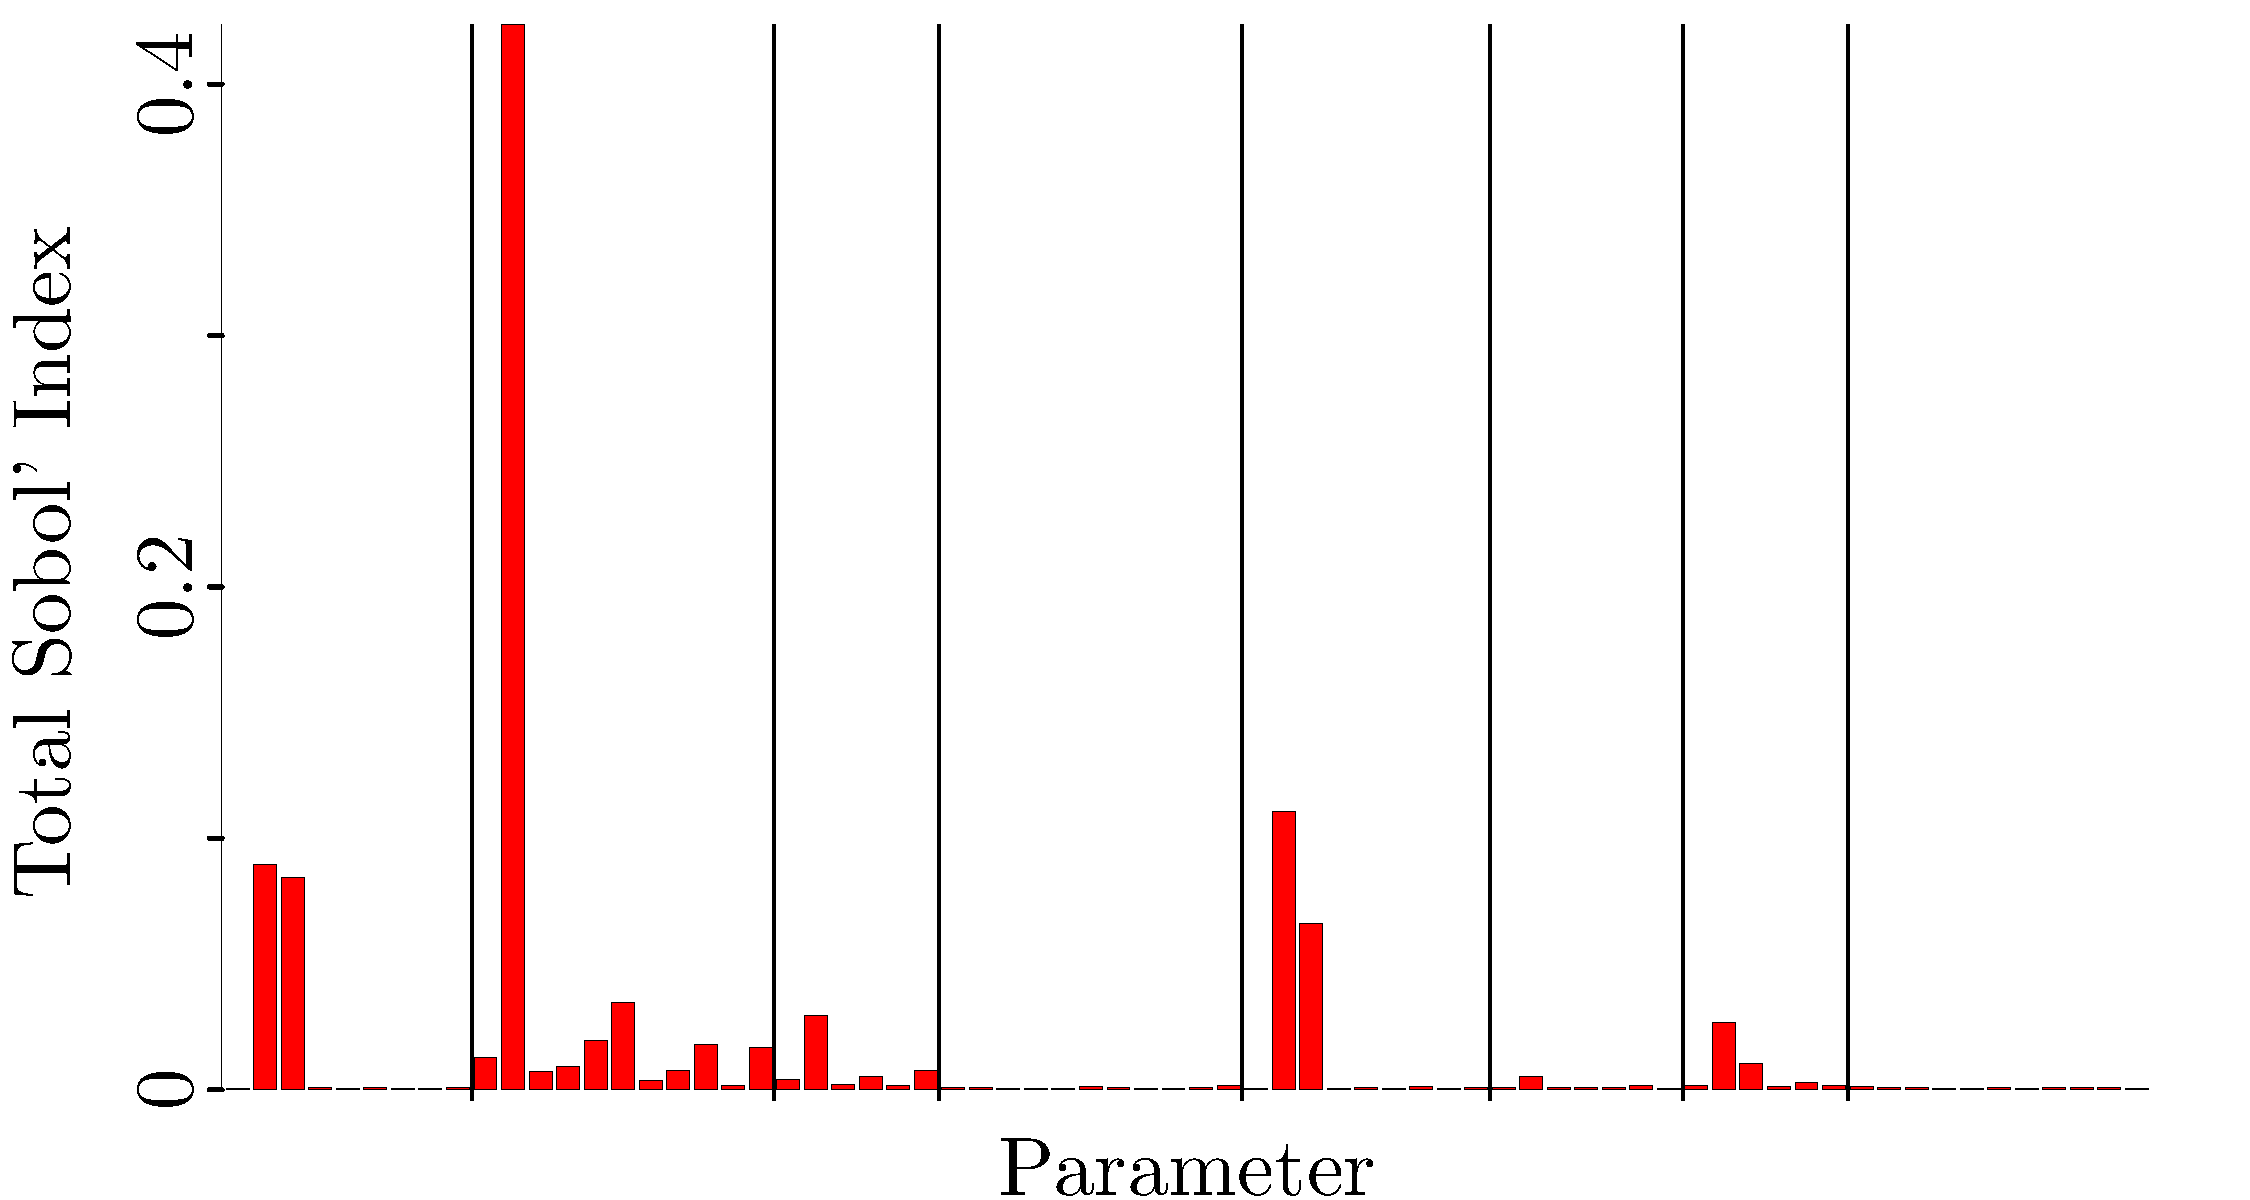
\includegraphics[scale=.25]{Figures/All_Parameters.pdf}
\end{center}
\caption{Total Sobol' indices for 70 parameters in the 8 channels. The black vertical lines are separating the channels. There are 13 parameters whose total Sobol' index is greater than 0.01.}
\label{fig:all_parameters}
\end{figure}

\begin{figure}[h]
\begin{center}
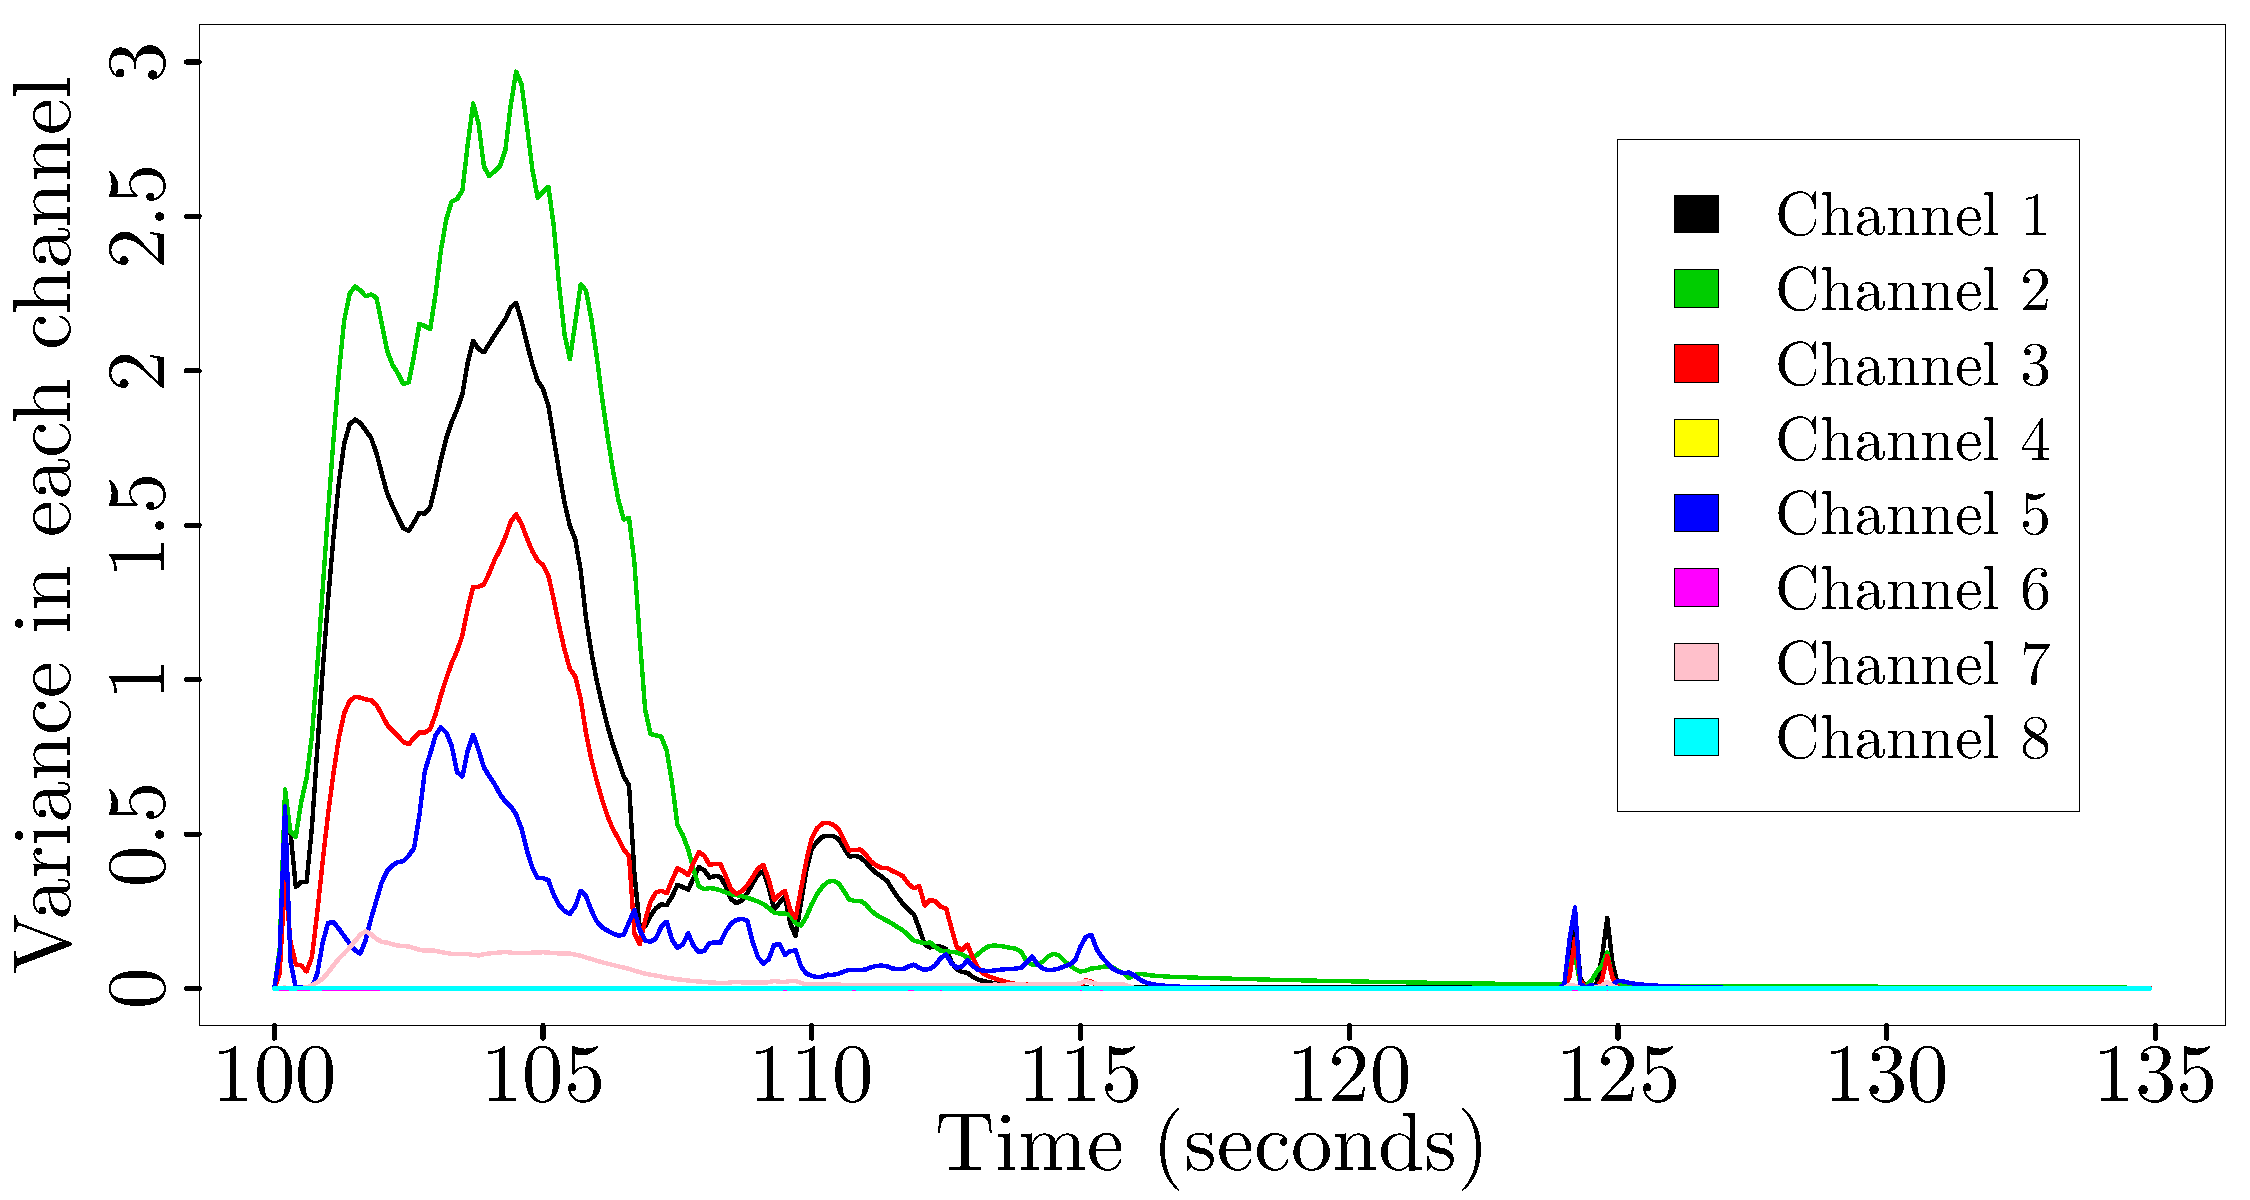
\includegraphics[scale=.25]{Figures/Channel_Variance_Comparison.pdf}
\end{center}
\caption{Variance of the $K_e$ profile when varying parameters within each channel and fixing others to their nominal values.}
\label{fig:channelwise_variances}
\end{figure}

\newpage

\begin{figure}[h]
\begin{center}
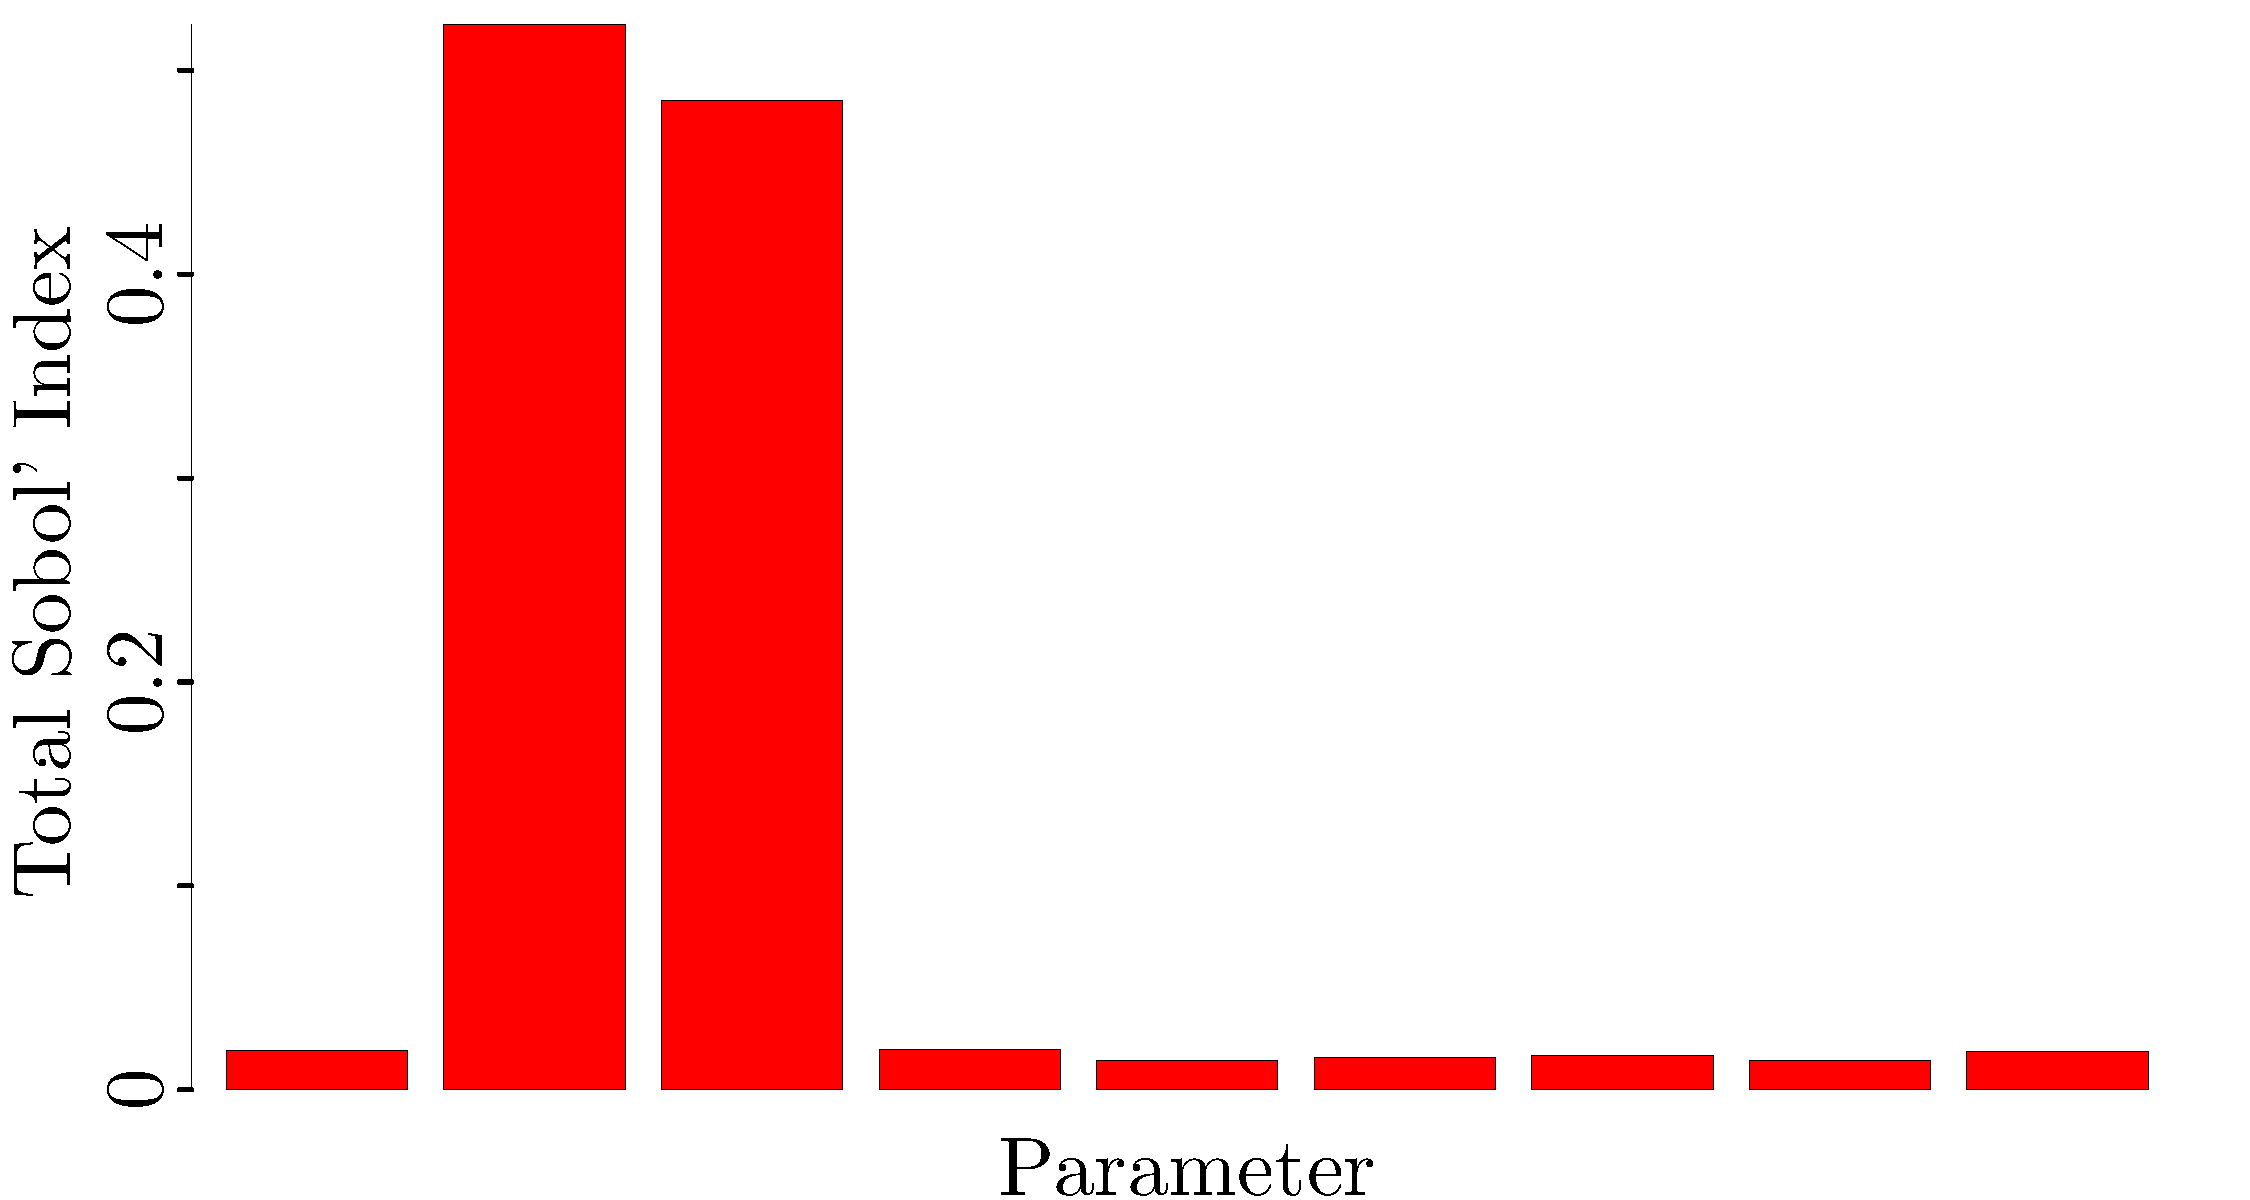
\includegraphics[scale=.2]{Figures/Channel_1_Parameters.pdf}
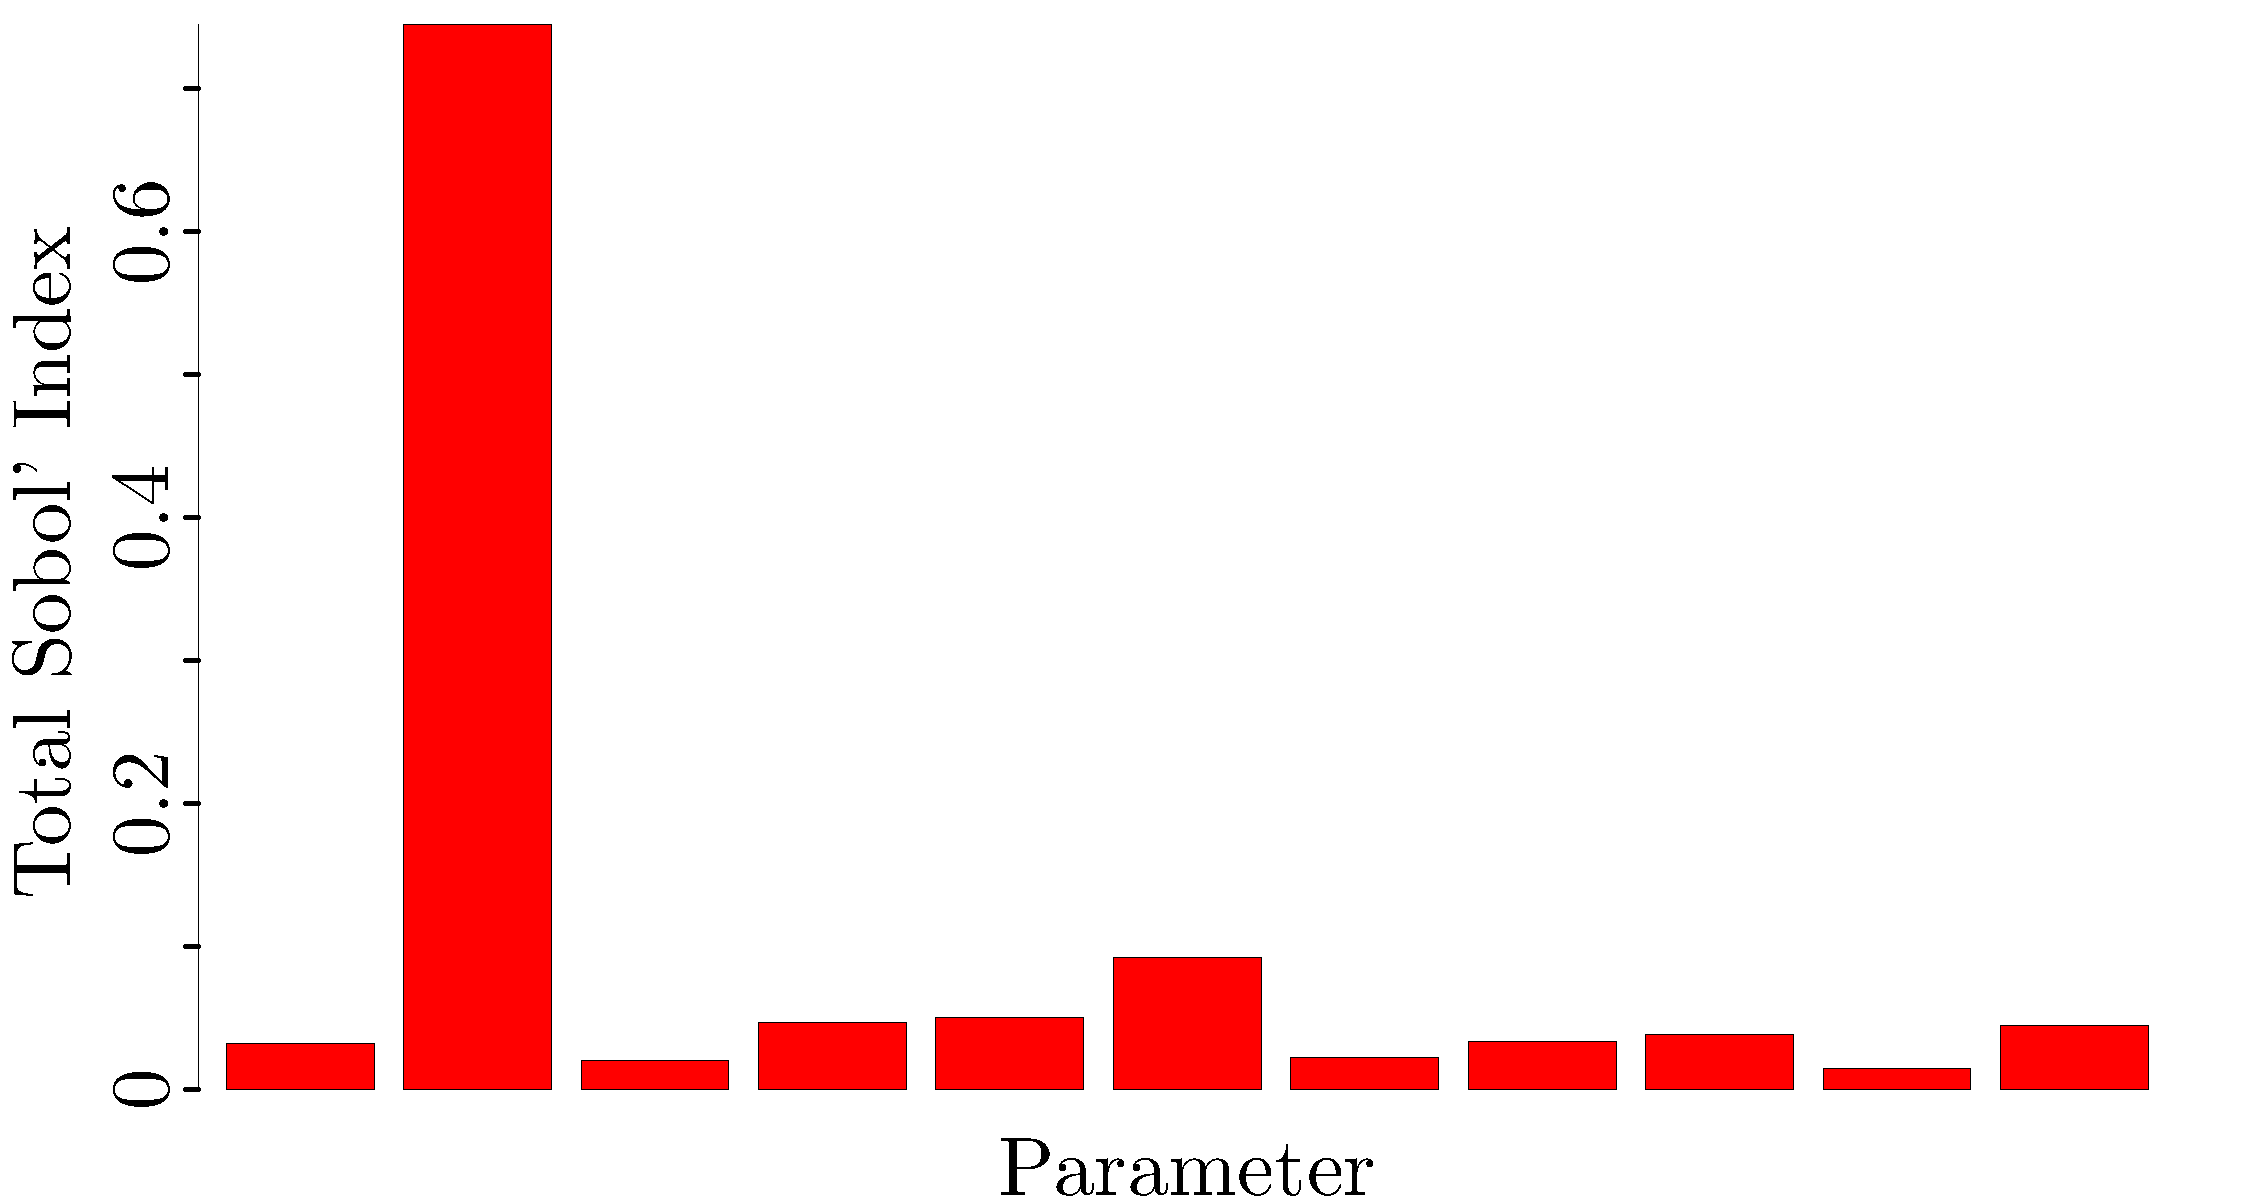
\includegraphics[scale=.2]{Figures/Channel_2_Parameters.pdf}
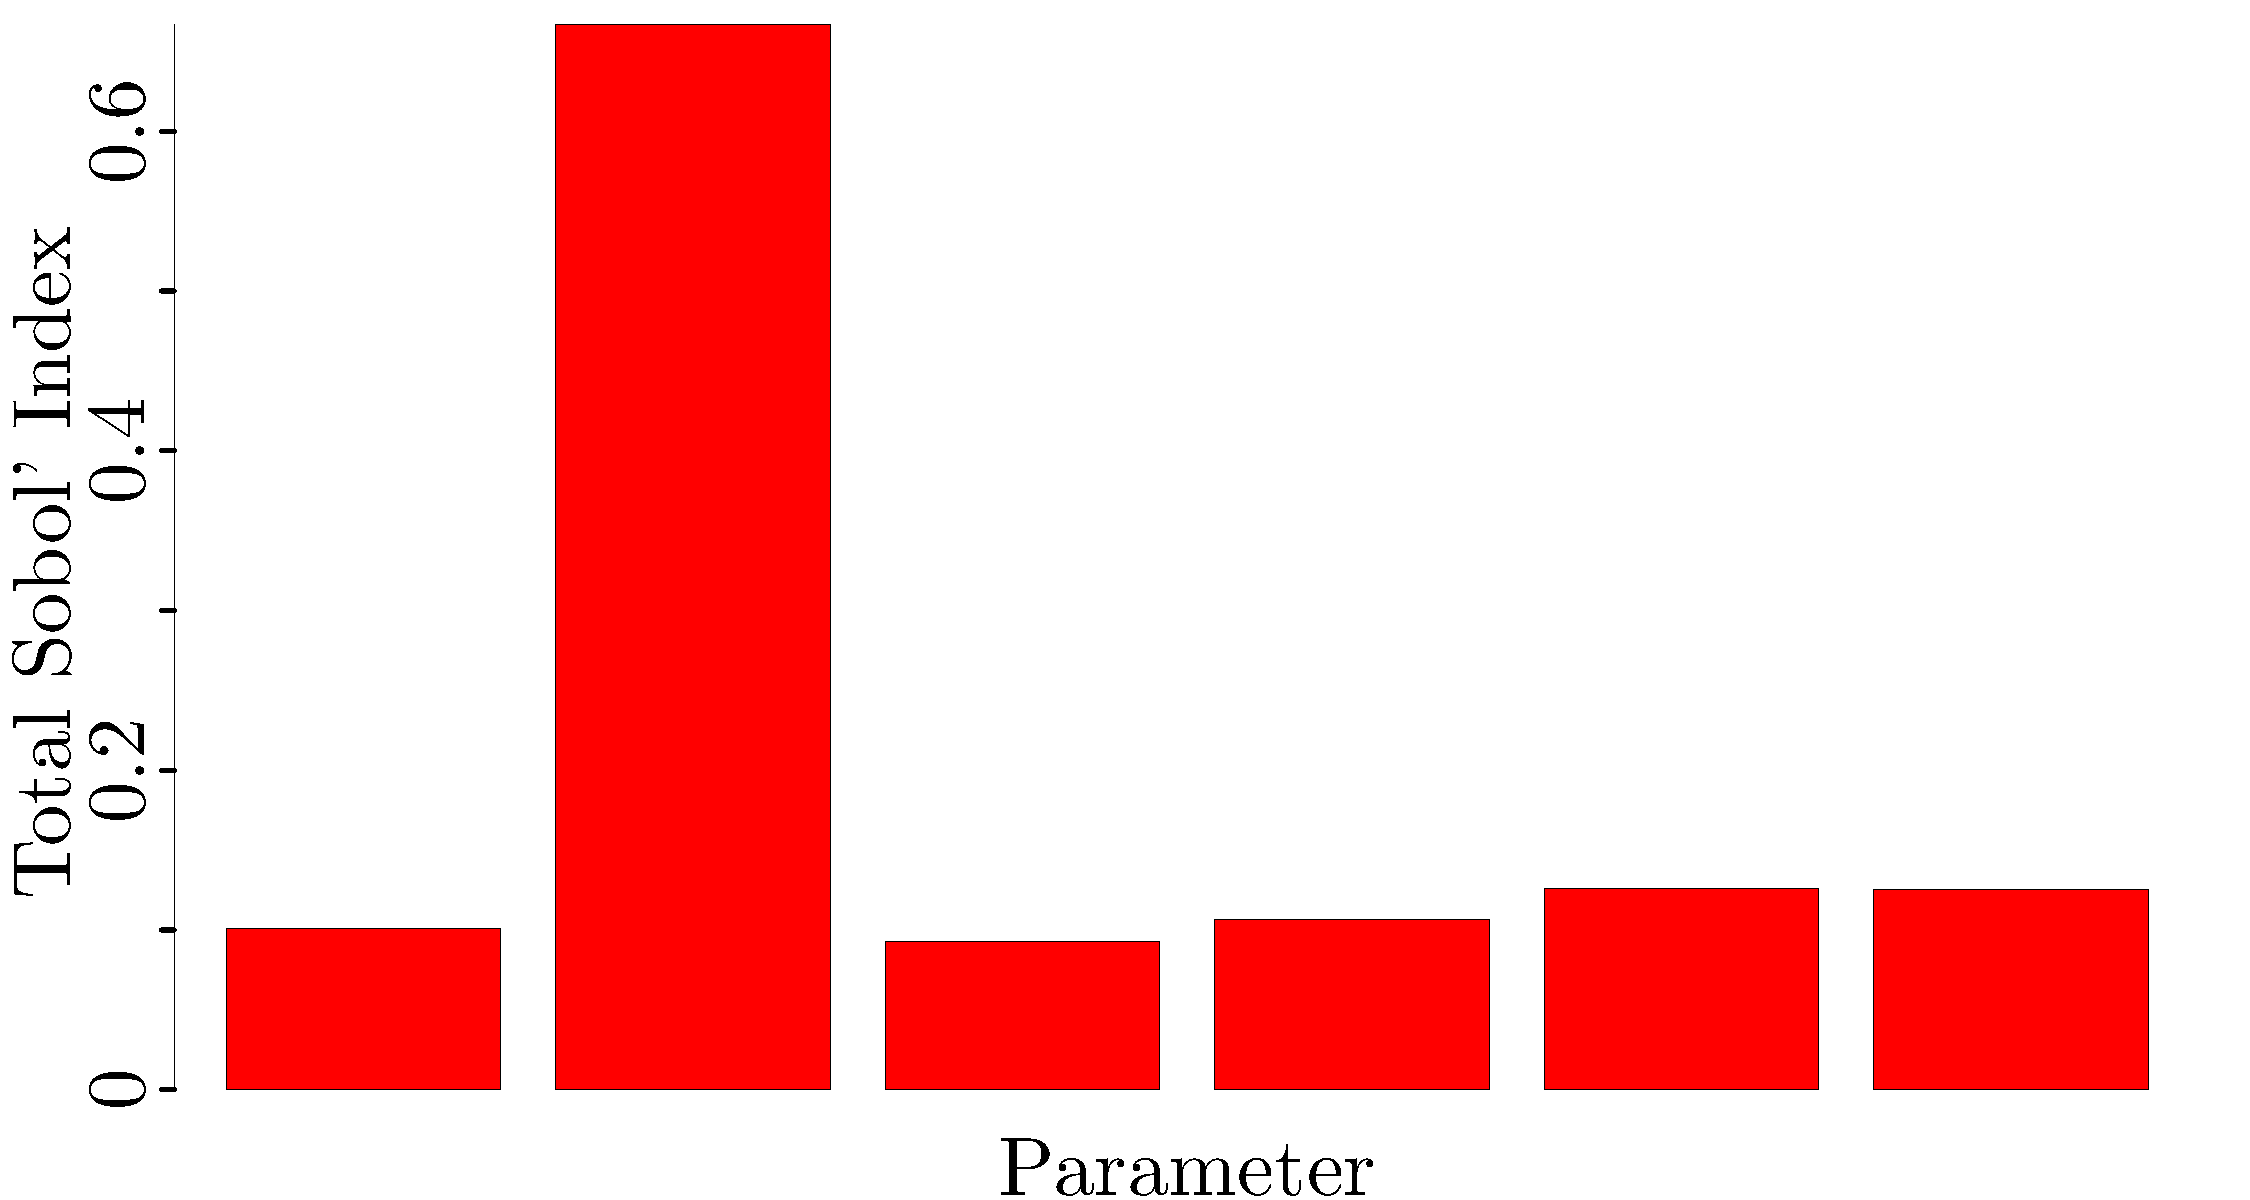
\includegraphics[scale=.2]{Figures/Channel_3_Parameters.pdf}
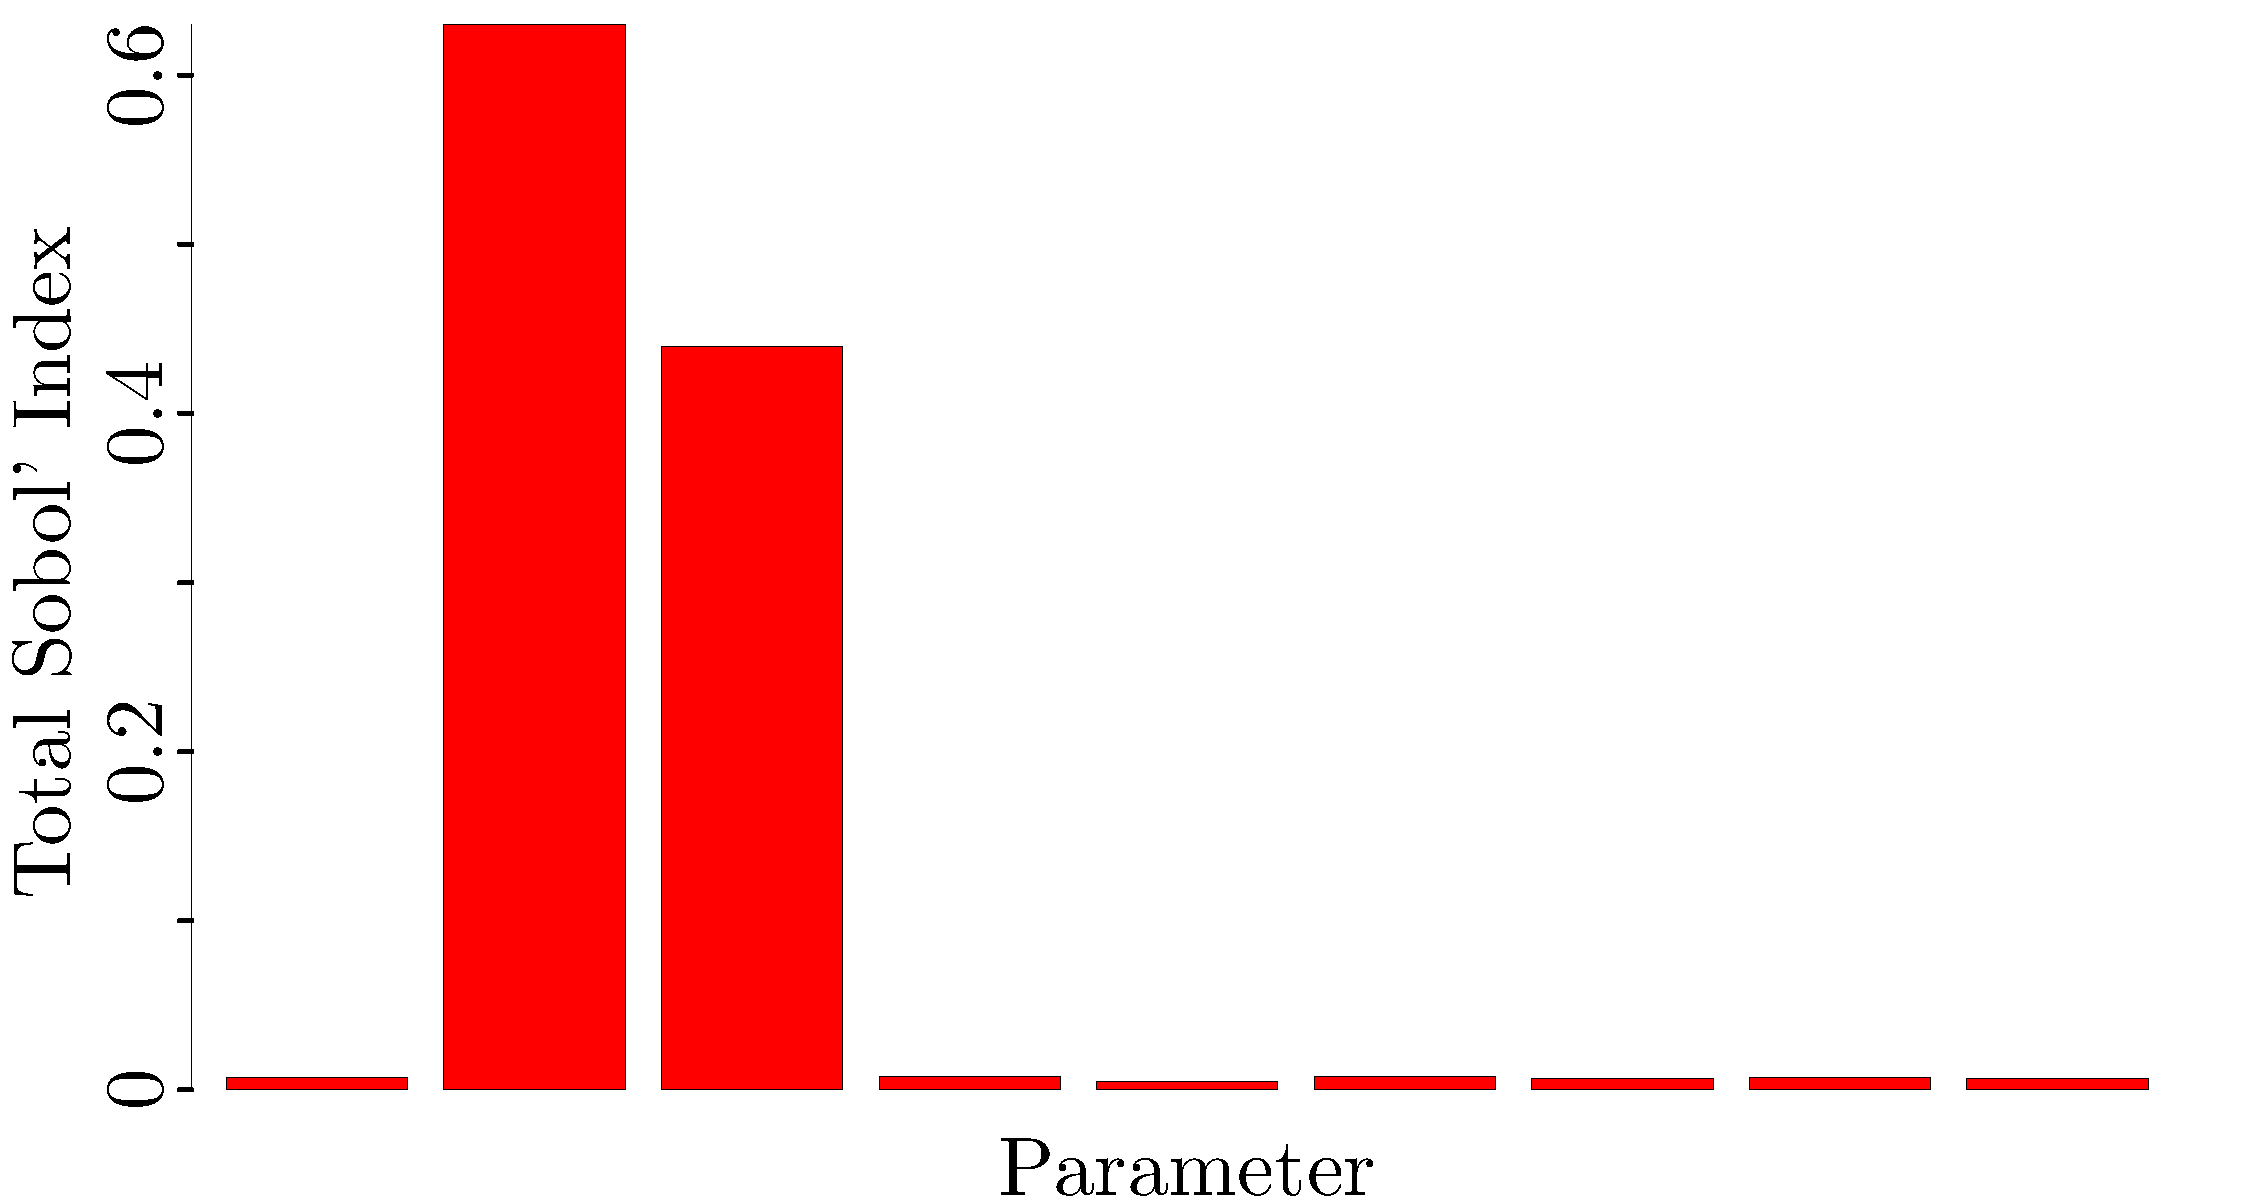
\includegraphics[scale=.2]{Figures/Channel_5_Parameters.pdf}
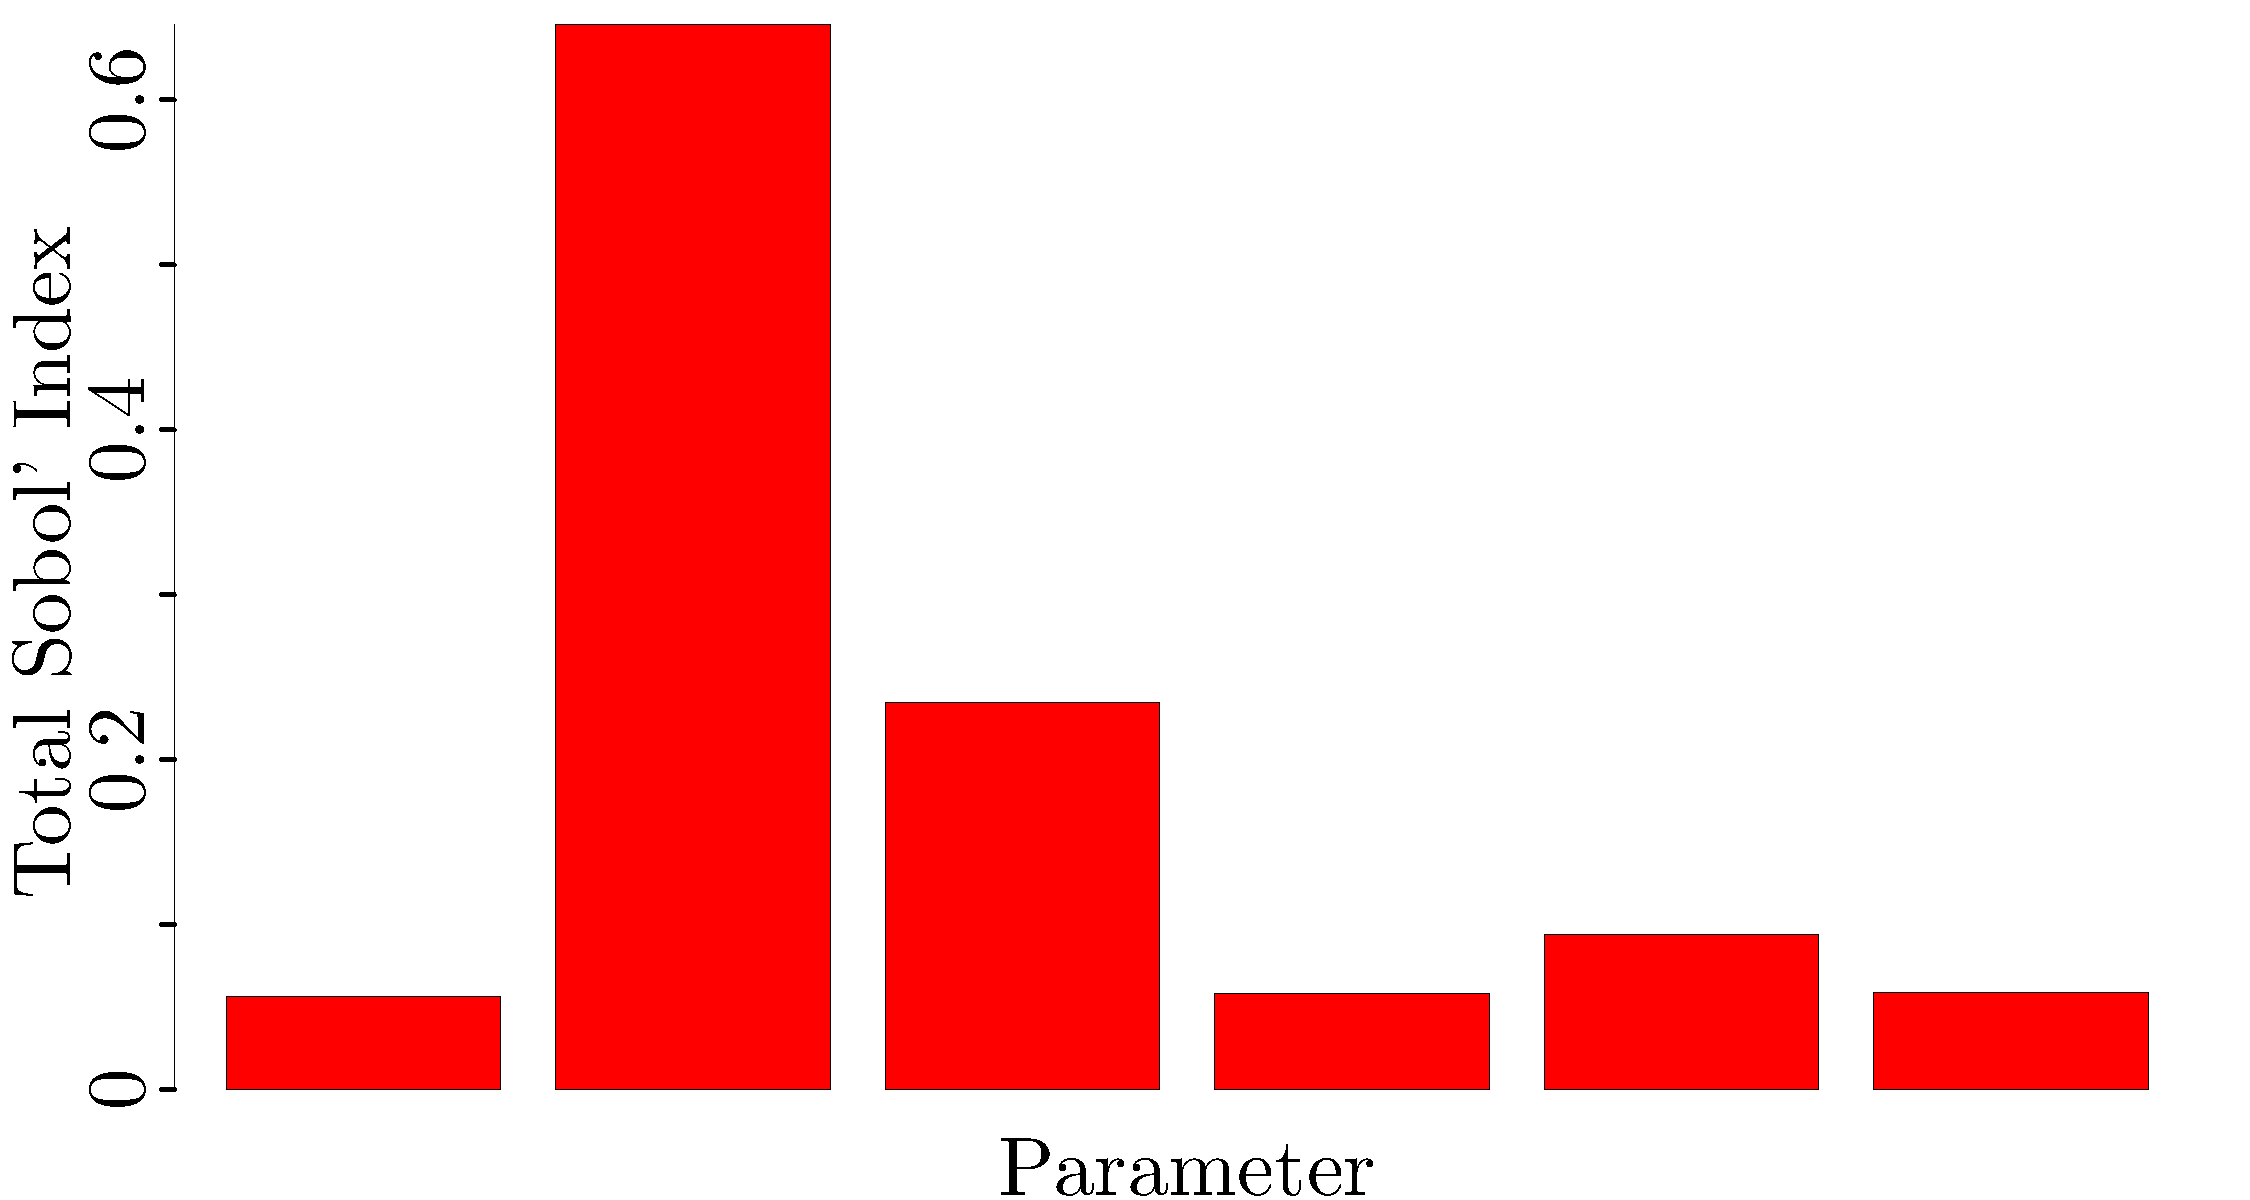
\includegraphics[scale=.2]{Figures/Channel_7_Parameters.pdf}
\end{center}
\caption{Total Sobol' indices for parameters in channels 1,2,3,5, and 7. Channel 1 is in the top left, channel 2 the top right, channel 3 the middle left, channel 5 the middle right, and channel 7 at the bottom. In each case all other parameters are fixed to their nominal values so these results ignore interactions of parameters across channels.}
\label{fig:channelwise_sobol}
\end{figure}


\newpage

Using the results of Figure~\ref{fig:all_parameters} we deduce that only 13 of the original 70 parameters should be varied. 

\section{NO Pathway notes}
\commTim{We also suspected that the NO pathway is influential so we perform a similar analysis on its parameters. There are 58 parameters which we vary, they are described in the document Tim wrote, "uncertainty\_quantification/Working\_Documents/Code\_Description/NO\_Pathway\_version\_2.pdf." We computed 1000 realizations and a subset of these are shown in Figure \ref{fig:CBF_Vary_NO_Pathway}. It is clear from this initial data set that increasing the influence of NO on NVC can provide a concave profile (top 3 realisation profiles) but the CBF profile does not reduce after the stimulus is finished and hence the second stimulus causes a much higher CBF than experiment suggests. This may be due to the rate of consumption of NO in the cells (particularly the SMC) or that the NO pathway is not the phenomenon that supports the concavity of the CBF profile. }

\begin{figure}[h!]
\centering
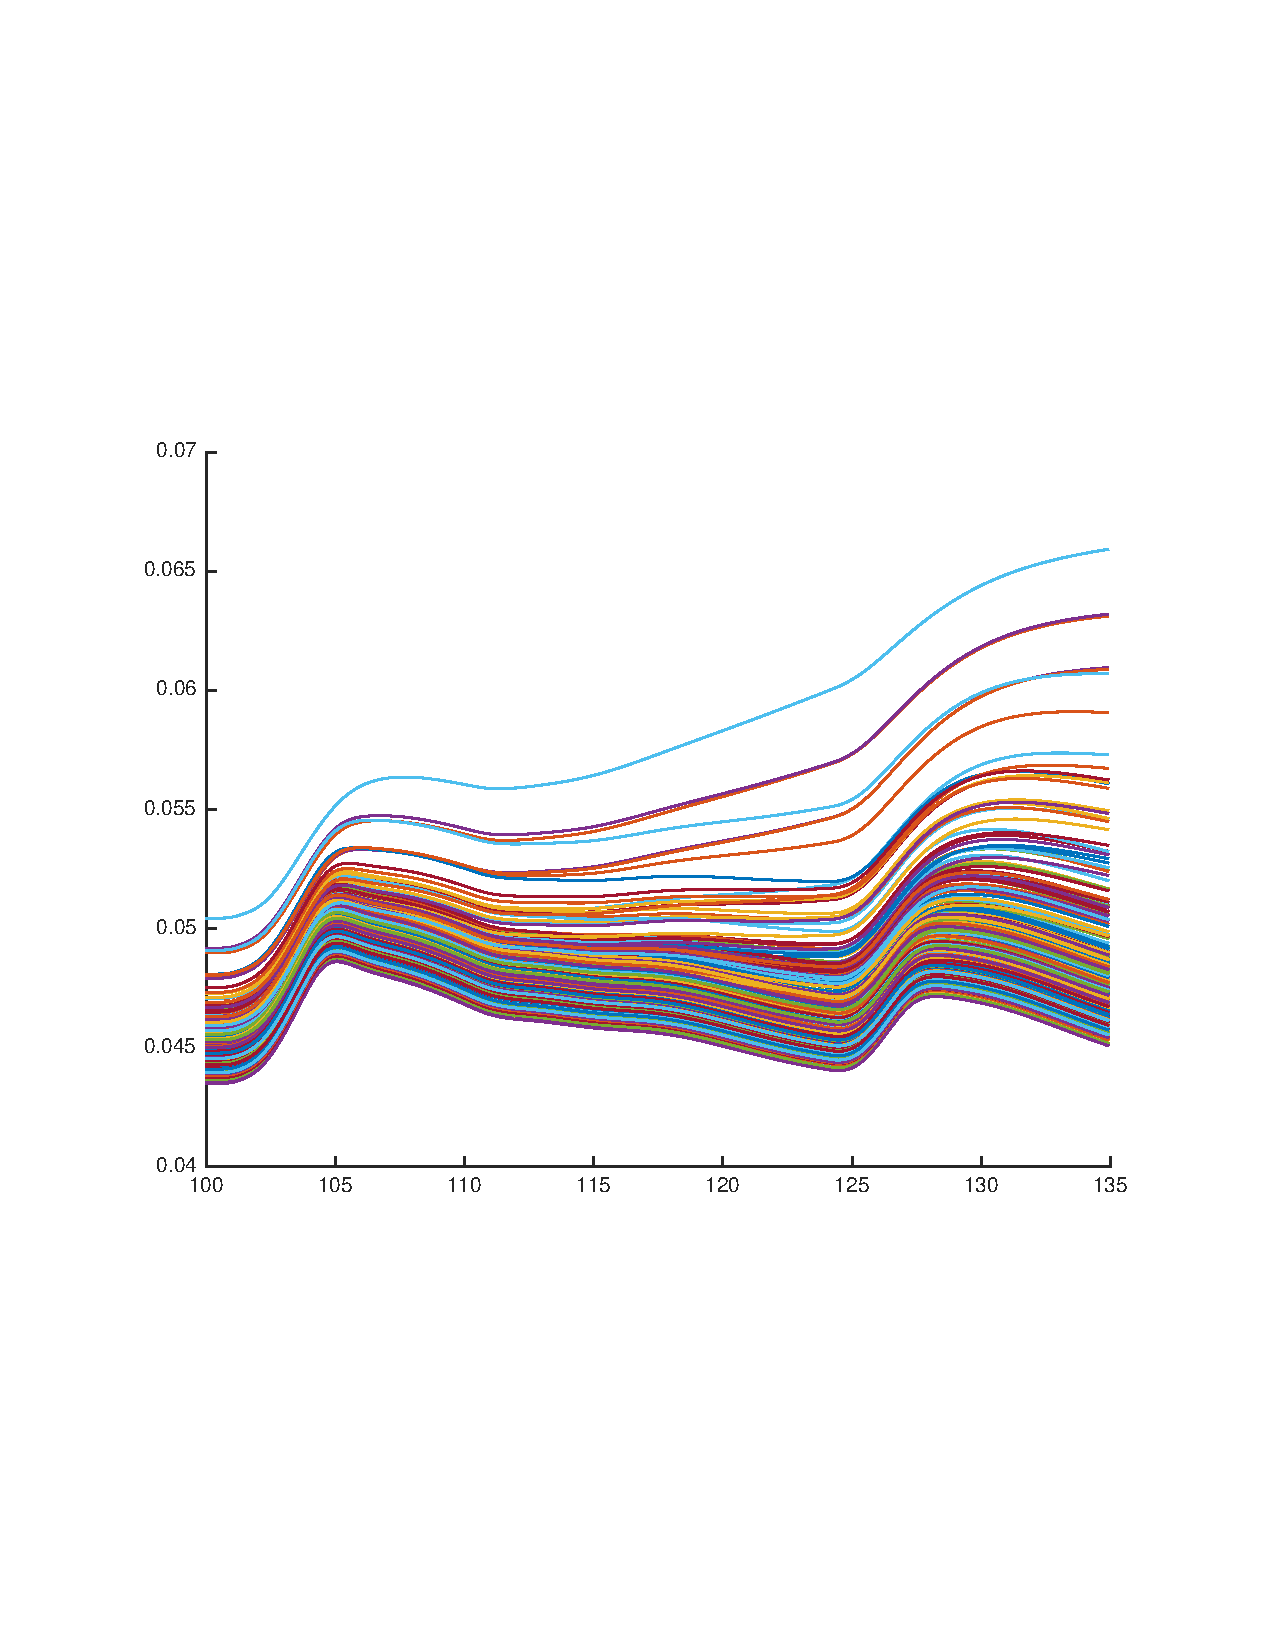
\includegraphics[width=0.8\linewidth]{./Figures/CBF_Vary_NO_Pathway}
\caption{CBF profiles from varying the 58 parameters defining the NO pathway from neuron to SMC and from EC to SMC.}
\label{fig:CBF_Vary_NO_Pathway}
\end{figure}

 From the 1,000 realisations we constructed a surrogate model using the KL expansion with radial basis functions. The Sobol' indices were computed using the surrogate model, they are shown in Figure~\ref{fig:NO_pathway_all_parameters}.

\begin{figure}[h]
\begin{center}
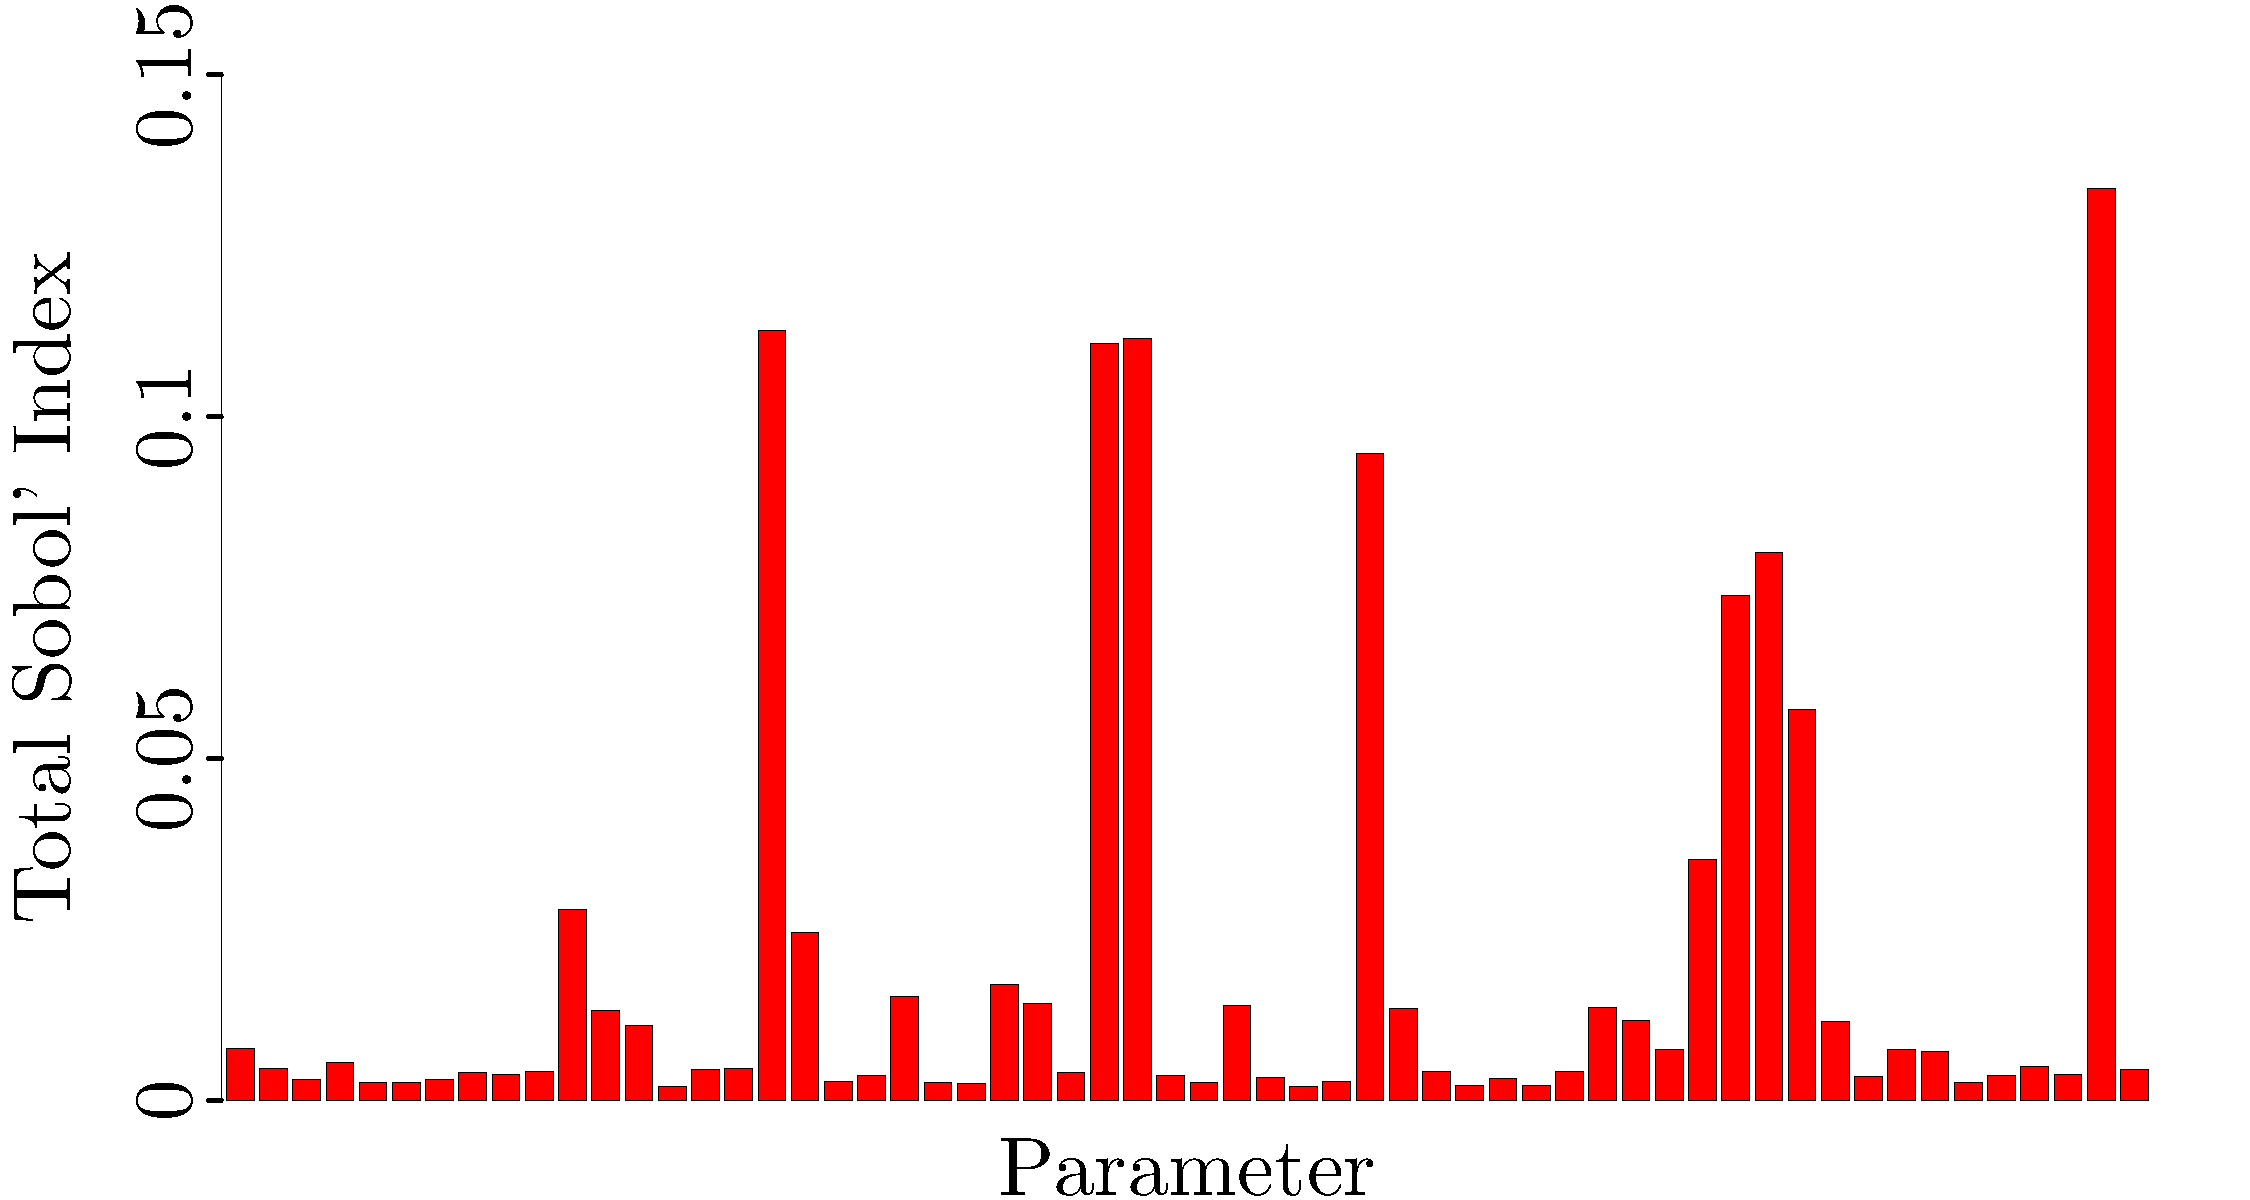
\includegraphics[scale=.25]{Figures/NO_Pathway_All_Parameters.pdf}
\end{center}
\caption{Total Sobol' indices for 58 NO pathway parameters. There are 11 parameters whose total Sobol' index is greater than 0.02 and 21 parameters whose total Sobol' index is greater than 0.01.}
\label{fig:NO_pathway_all_parameters}
\end{figure}

The 11 most influential parameters, in order, are
\begin{enumerate}\label{ranked_list_NO_parameters}
\item ('$x_{ki}$', 25);  [um];  (M.E.) in SMCEC
\item ('$x_{nk}'$, 25);             [um] ;  (M.E.) in Neuron
\item ('$x_{ki}$', 25);             [um] ;  (M.E.) in Astrocyte
\item ('$x_{nk}$', 25);             [um] ;  (M.E.) in Astrocyte
\item  ('$K_{m_{mlcp}}$', 5.5);  [uM] ; in SMCEC
\item ('$k_{pde}$', 0.0195);  [$s^{-1}$] ; in SMCEC
\item  ('$V_{max_{sGC}}$', 0.8520);  [] ; in SMCEC
\item ('$C_4$', 0.011);  [$s^{-1} microM^{-2}$]  in SMCEC
\item ('k3', 3);  [$uM^{-1} s^{-1}$] ; in SMCEC
\item ('$V_{max_{NO_{n}}}$', 4.22);     [$s^-1$] ; maximum catalytic rate of NO production (Chen2006) - obtained from fig 6 and equ 17 and 18 in Neuron
\item ('$D_{cNO}$', 3300);          [$um^2 s^-1$] ; Diffusion coefficient NO (Malinski1993) in Neuron
\end{enumerate}


\commTim{ From the list of ranked parameters above the consumption rate component does not have a large (or really any) influence on the profile so any solution to the "inverse" problem of finding a set of parameters which has a minimum sum of squared errors to the desire concave CBF profile would not involve NO consumption.\\
 From this we can perhaps hypothesise that NO is \textbf{not} the phenomenon which supports a concave CBF profile. So if not what is ?  \\
\textit{ It is interesting to note that the highest ranked parameters affecting the NO profile are the assumed (model estimated) distances of neuron to astrocyte, astrocyte to SMC and EC to SMC.}\\
There are a number of possible areas that we  investigate , itemised below\\
\begin{itemize}
\item an increase in the neuronal activation based on a delayed appearance of cortical activists such as dopamine or norepinephrine (noradrenaline) indicating a possible stress situation of the animal. 
\item different pathways from the whisker pad to the somatosensory cortex via the brainstem take different times (there is little if any evidence for this) 
\item long stimulation times cause an as yet unknown increase in neuronal activity
\item following Elizabeth Hillmann's hypothesis that upstream information is passed to the pial arteries from the parenchyma which then respond (dilate causing increased flow) after a certain time. 
\item LDF probe used in the data of Zheng et al \cite{Zheng2010} was described as \textbf{The LDF probe (PeriFlux 5010, Perimed, Stockholm, 780 nm illumination, 0.25 mm separation) was placed under visual guidance (Leica MZ 7.5 stereomicroscope—×60 magnification) such that it overlays the cortical surface ( less than 1 mm) and that the maximum
distance from the LDF probe to the uppermost channel of the multichannel electrode was approximately 100 μmin the x–y plane.} So this means that the CBF profile is an average of both penetrating arterioles and the pial arteries. 
\item low frequency oscillation (0.1 Hz) caused by dynamics of the relationship between CICR, SERCA and RyR may be initiated after a short period of 8 seconds. 
\end{itemize} 
The fact that the CBF is measured above the cortex indicates that the CBF is an average of a number of arterioles and the pial arteries. Thus Hillman's work \cite{Chen2014a} on the endothelial mediated transfer upstream of dilation to the pial arteries could be a possible explanation. In fact when they use acetacholine (ACh) to predilate arteries see supplementary figure S5c the change in HbT shows distinctive "concave" -like profiles. The addition of ACh would also induce significant amounts of $Ca^{2+}$ from the stores via the G -protein coupled receptor (which would initially constrict the vessels). If the ACh concentration is within a specific range then the SMC may oscillate at approx 0.1Hz. Therefore we should look at the work of Johny et al \cite{Johny2017} to investigate whether the agonist can produce oscillations which may simulate the concavity profile of the CBF. This does not negate the role of Hillman's hypothesis.\\
Talking with KC Brennan and colleagues it seems possible that the concavity is induced by \textit{neuronal modulation}. This is where agonists such as ACh or norepinephrine are released in the somatosensory cortex. This release of agonist then diffuses through the cortical tissue and would increased neuronal activation along with possible cellular oscillations as noted above. \\
 The sketch shown in Figure \ref{fig:Neuromodulation_paths} provides a viable hypothesis. }
\begin{figure}[h!]
\centering
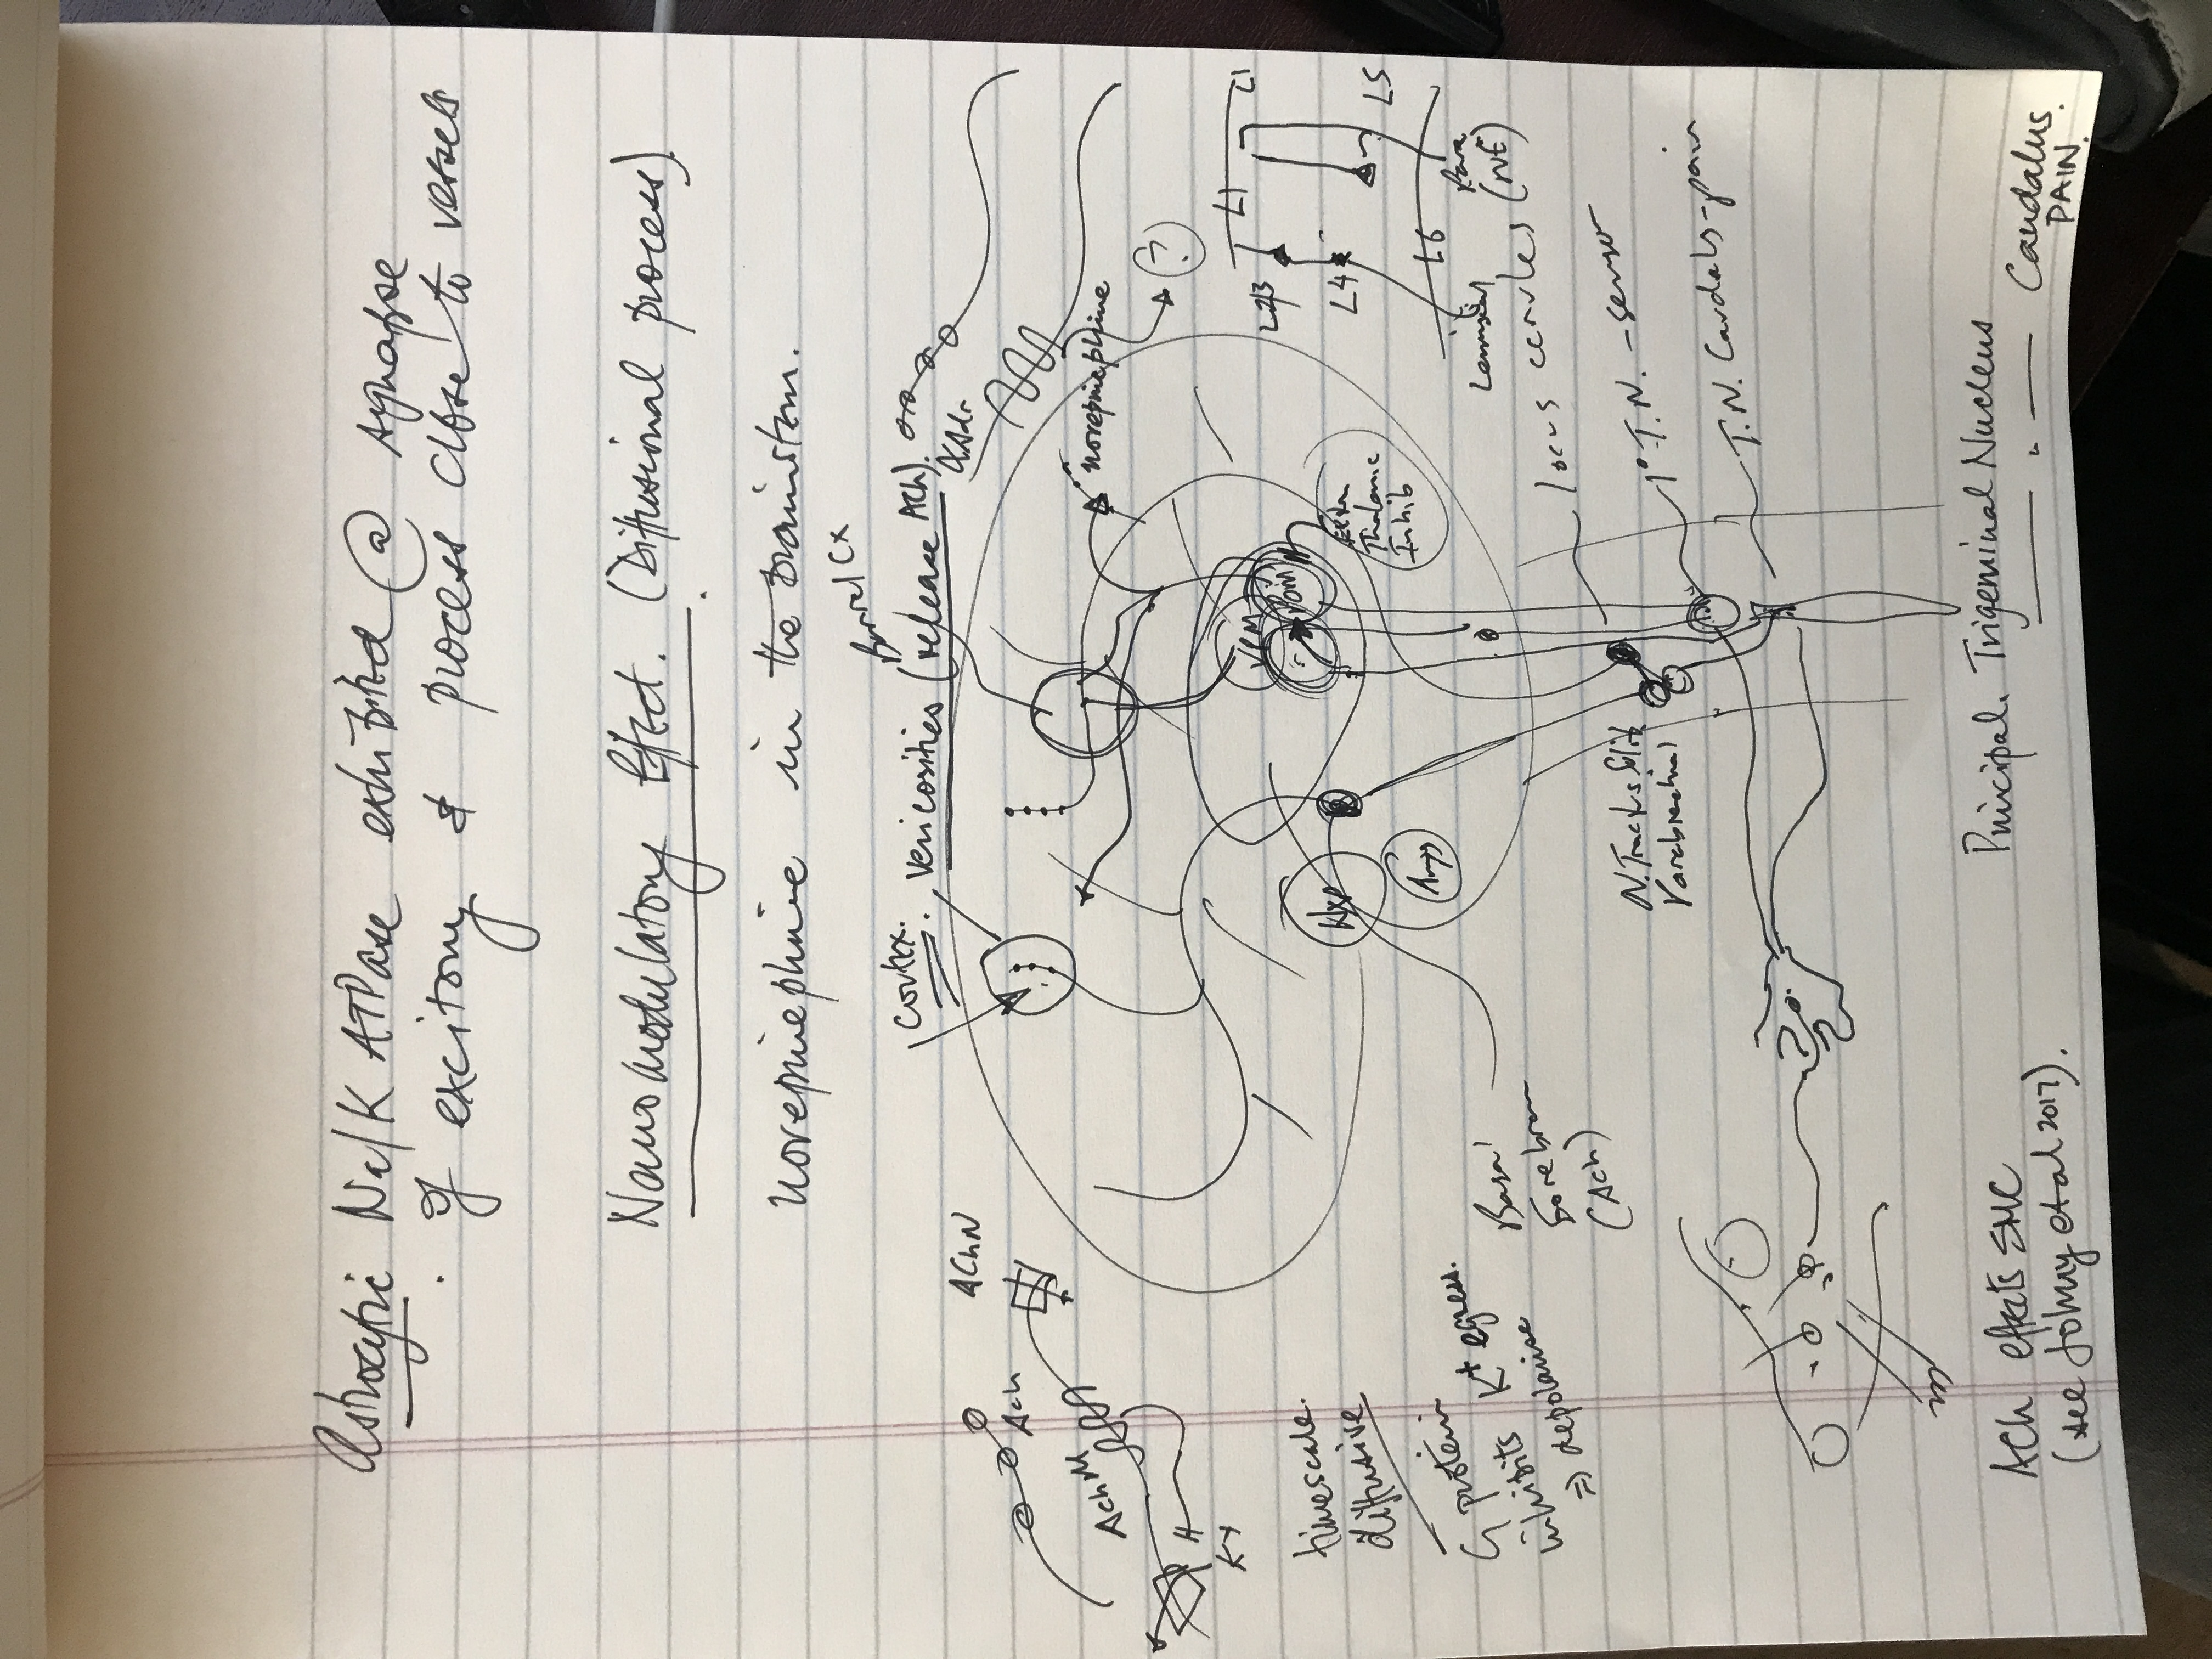
\includegraphics[width=0.7\linewidth, angle = -90]{./Figures/Neuromodulation_paths}
\caption{Sketch of neuromodulation paths for ACh and Norepinephrine}
\label{fig:Neuromodulation_paths}
\end{figure}
\commTim{Berwick's group suggest that the concavity of the CBF is based on competing dilatory and constricting phenomena. Dilation  by EPSP (excitory post synaptic potential) and constriction by IPSP (inhibitory post synapyic potential). I can't find any evidence to support this.  The basis of the contrasting hypothesis is that for long stimulations, ($\ge 8 secs$)  the path from the whisker pad mediates a neuromodulatory effect for both ACh and norepinephrine (directed through both the locus coeruleus and the nucleus tractus solitarius to the hypothalamus bypassing the VPM and POM in the thalamus) and provides for the release of these agonists in the sensory cortex.
%through the Principal Trigenimal Nucleus to the VPM (ventral posteromedial nucleus  is a nucleus of the thalamus) and thence to the somatosenory cortex allows ACh to efflux through the vericosities that exist on the dendrites of layer 2/3 neurons (calbindin-immuno-reactive neurons (CIR neurons)).
 This release of ACh, for example then diffuses through the cortical tissue and mediates a dilation of vessels cerebral arteries appear to have M5 muscarinic receptors that produce vasodilation in response to ACh. But this response is due to the probable release of endothelial derived NO !!! This then leads to an increase in CBF. Due to the slow  kinetics of this process the ACh mediated dilation will not immediately become apparent.  The input data from Berwick's group was current source density measurements in layer IV and this showed no increase in activity, we could argue that the neuromodulatory effect is seen mostly in layer 1,2,3. \\
 KC's comments make it clear that the original input current from the stimulus should not be altered but that neuromodulation is an additional neuronal activation. Unfortunately we do not know what the time dependent profile of neuromodulation  would be like.\\
% How do we model the time dependent behaviour of a neuromodulatory effect (of ACh and Norepi) which essentially releases endothelially derived Nitric Oxide?\\
 Work by Edith Hamel (in Montreal) has given us the experimental evidence we need \cite{Toussay2013}. This paper provides evidence of noradrenaline cortical activation through the Locus Coeruleus. It provides basic pathways which include the cAMP and PIP2 pathways for neuronal $Ca^{2+}$  as well as nNOS. We can therefore provide an additional pathway to the "standard" neuronal activation. Hamel's work shows the timescales  over which the noradrenaline pathway is active. We shall call this the Pain pathway\\
 \textbf{Notes on some possible models of the Pain pathway.}\\
 Hamel's group states  "\textbf{...that LC stimulation recruits a broad network of cortical excitatory and inhibitory neurons resulting in increased cortical activity and that K?fluxes and EET signaling mediate a large part of the hemodynamic response.}". They further state that "\textbf{LC activates a broad network of cortical pyramidal cells and interneurons and concomitantly increases cortical perfusion. The hyperemic response virtually disappeared after selective lesioning of the LC–NA system and required activation of $\alpha$ - and $\beta$ -adrenoreceptors. In addition, the evoked CBF response to the LC-NA system required the release of glutamate and GABA likely from the recruited subsets of pyramidal cells and interneurons and was primarily mediated by epoxyeicosatrienoic acids (EETs) and potassium ($K^+$) fluxes through large- conductance, calcium-operated (BK) and inward-rectifier (Kir) $K^+$ channels.}"\\
 Stimulation consisted of "\textbf{of 10 bursts of pulses (100 Hz, 0.5 ms duration) presented at 0.5 Hz (1 s on/1 s off for a total of 20 s) with a current intensity of 80$\mu$ A.}" CBF measurements were done using LDF 100 $\mu$m probes . From the Toussey paper it is clear that both $K^+$ , $K_{IR}$ and neuronal NO pathways have an influence. In addition in the work by Toussey et al \cite{Toussay2013} mean arterial pressure (MAP) increased during LC stimulation, however the Zheng experiment \cite{Zheng2010} used Phenylephrine infusion to keep MAP constant.  \\
 After much thought (!) it seems th ebeat way of modelling this (albeit rather phenomenologically ) is to split the stimulation current that is applied to the neuron compartment into two parts, as given by 
 
 }
 \begin{eqnarray}
 I_{T}=\alpha I_{LC}(t)+\beta I_{Wh}(t)
 \end{eqnarray}
 \commTim{here $I_{LC }$ is the current coming from the locus coeruleus and $I_{Wh}$ from the whisker pad through the Principal trigeminal  nucleus; $\alpha$ and $\beta$ are weighting parameters. They are assumed to be essentially independent pathways. We show this in Figure \ref{fig:LC_Wh_pathways}. 
  }
 \begin{figure}[h!]
\centering
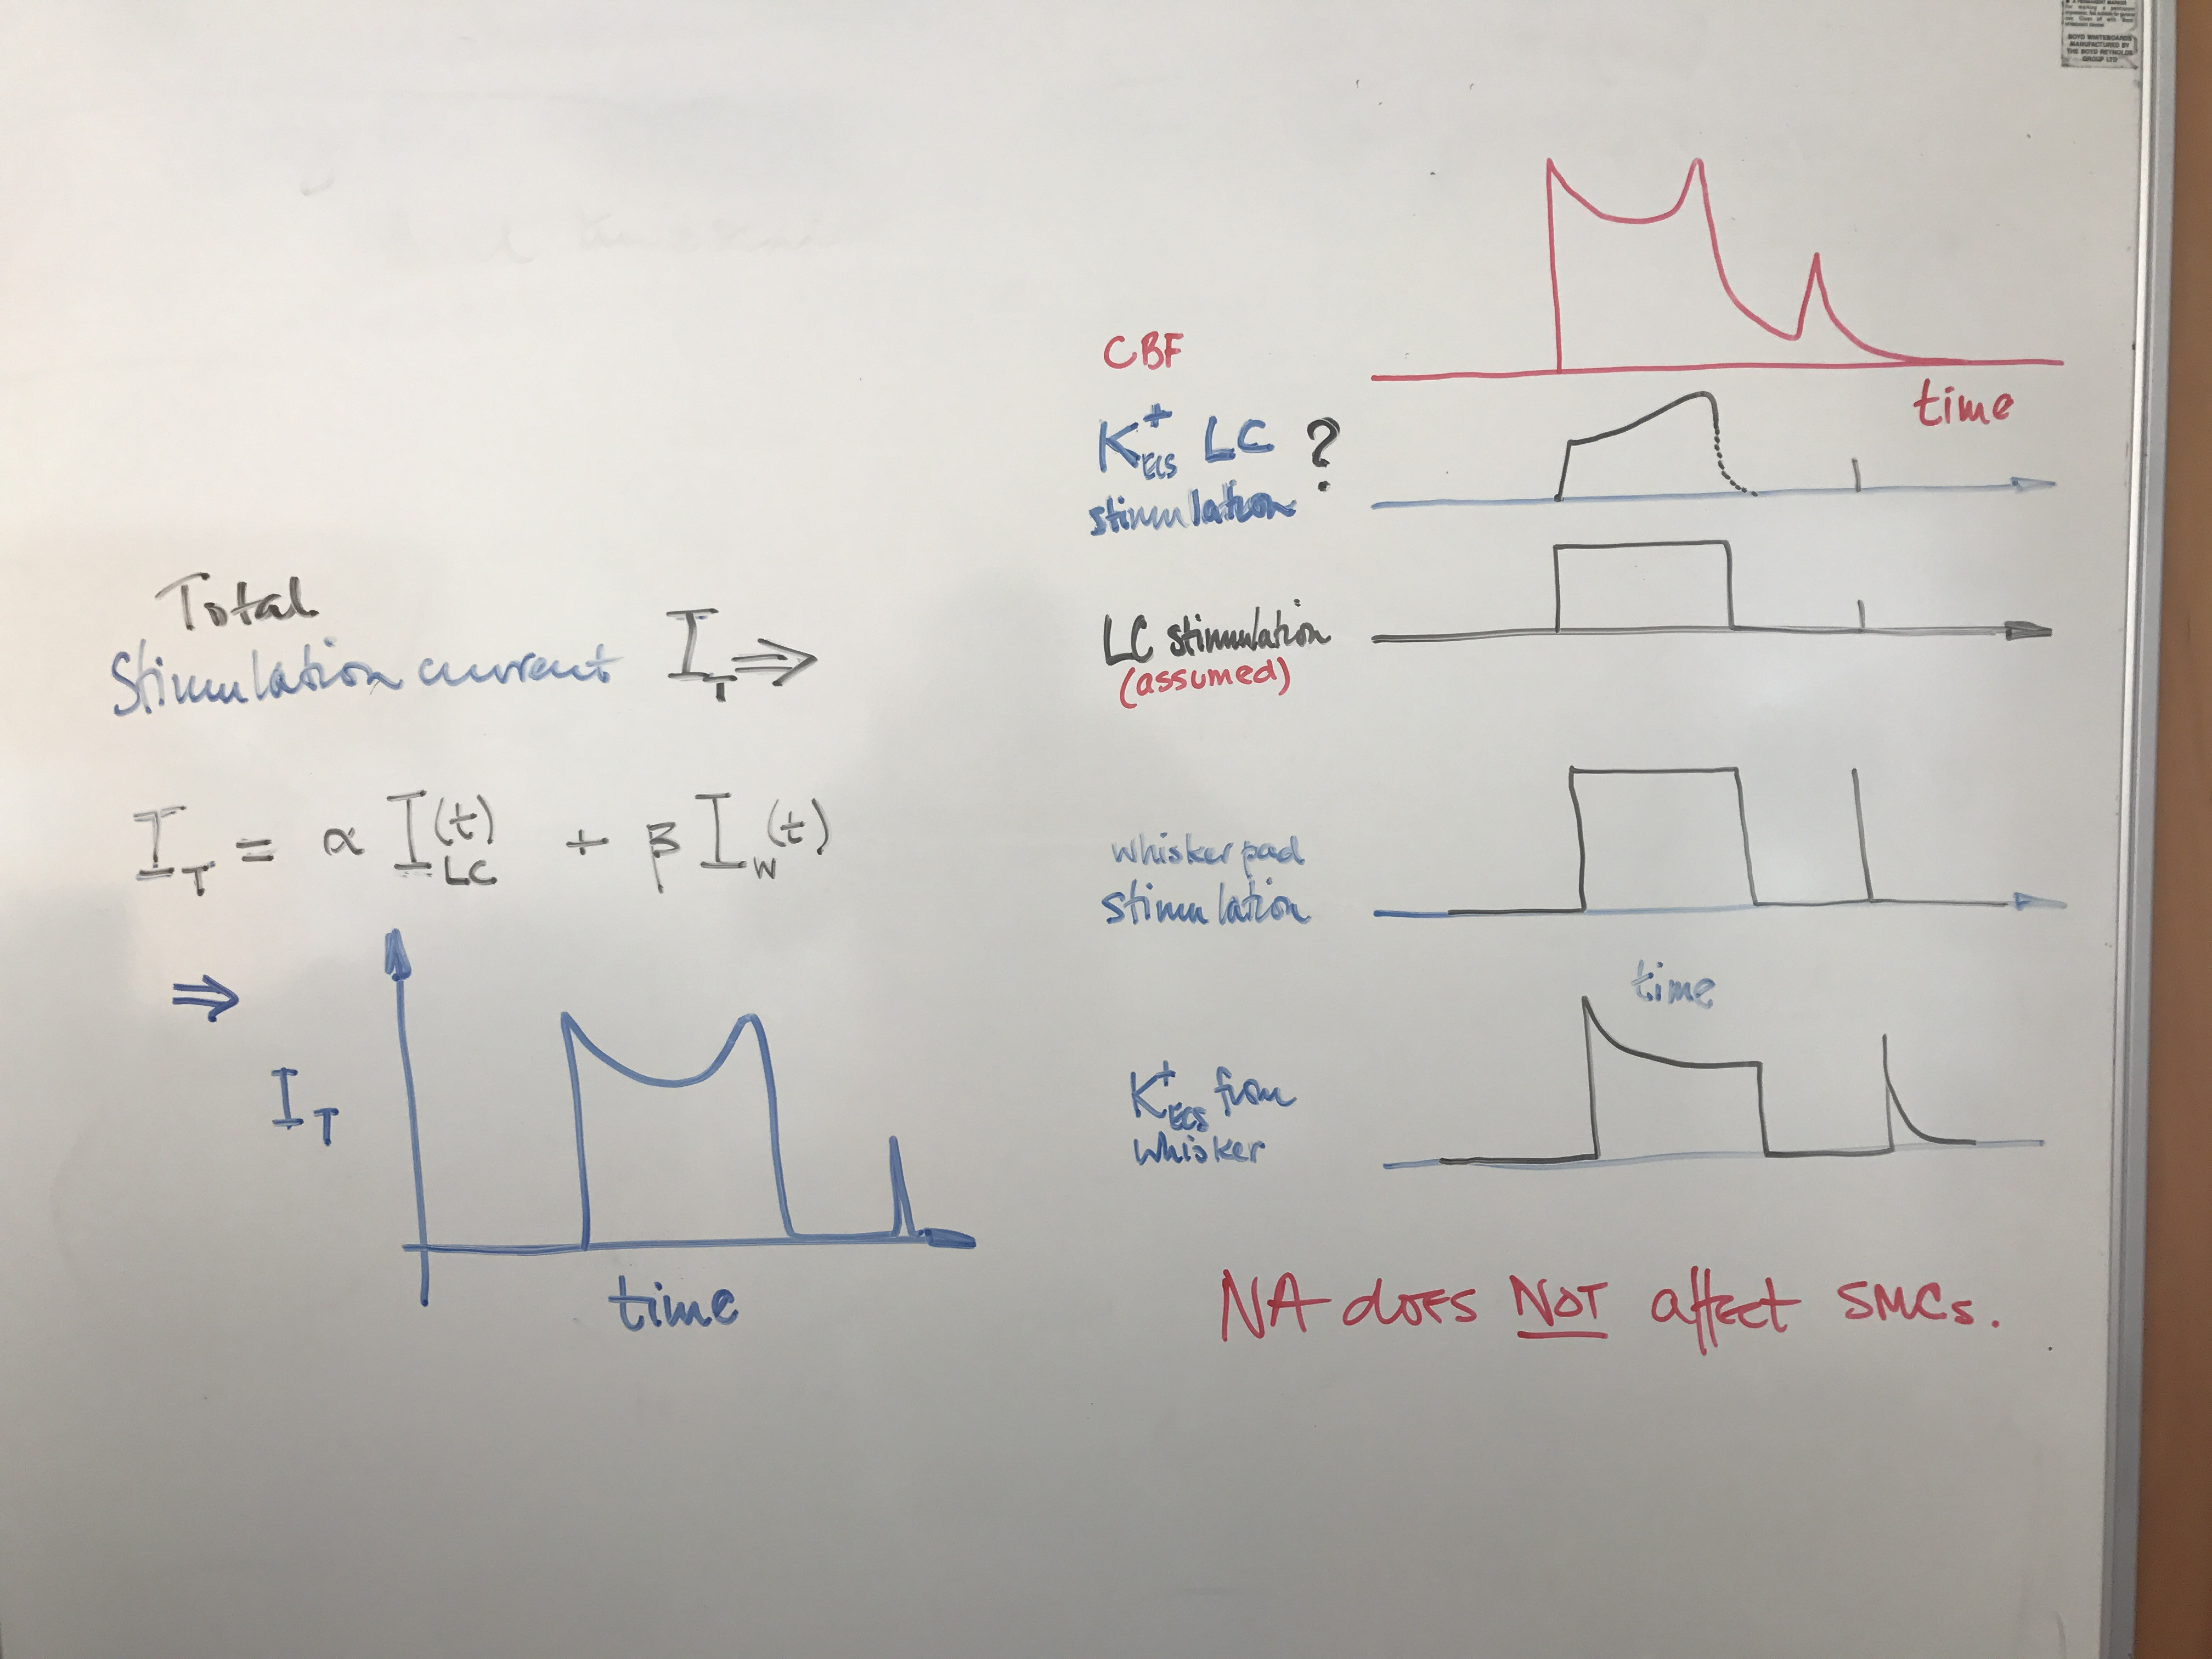
\includegraphics[width=0.7\linewidth]{./Figures/LC_Wh_pathways}
\caption{A sketch of the combined effect of the LC and "standard" whisker pad currents}
\label{fig:LC_Wh_pathways}
\end{figure}
\commTim{\section{Analysis of various pathways in the NVU}
In comparing the neurovascular coupling results to experiment (specifically murine experiments) it is clear that the time taken for the perfusing vessel to react is slow. Previous work (\cite{Kenny2017}) has shown that there are a number of pathways which influence the neurovascular coupling, especially the change and rate of change of the radius of the perfusing vessel. We therefore wish to analyse not only which pathway has the most influence but also which set of parameters that define the specific pathway have a significant influence on the vessel dynamics. 
Currently we look at three different pathways.
\begin{enumerate}
\item NO 
\item $K^+$ 
\item $Ca^{2+}$ in the EC/SMC coupling
\end{enumerate}
We will not look at the TRPV4 channel at this time. 
A list of parameters which affect the three pathways have been defined (and highlighted) in the code. These parameters (as done previously) will be assigned mean values and a uniform distribution ($\pm$ 10 \%). 
Figure \ref{fig:inputoutput} shows a sketch of the input (current into the neuron $I_{m}$, non-zero over the interval ($t_0,t_1$) and a profile of the vessel radius change as a function of time.   
\begin{figure}[h!]
\centering
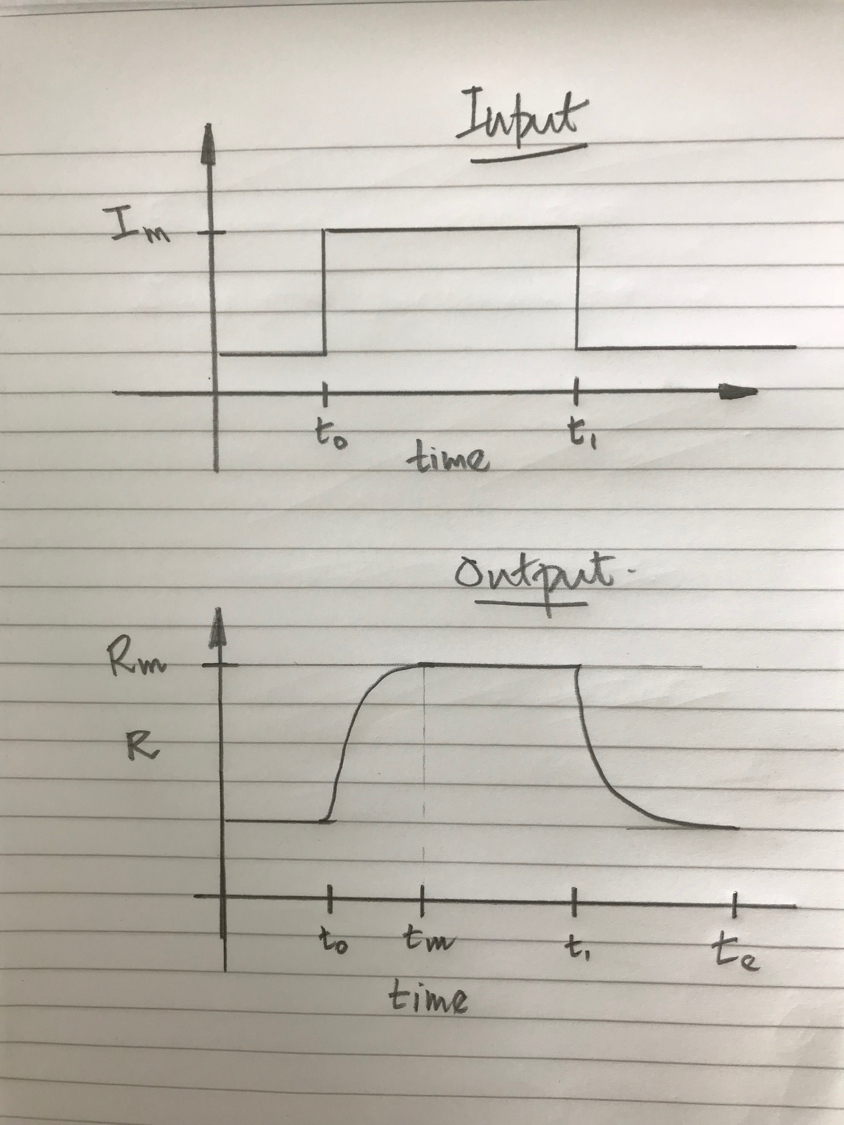
\includegraphics[width=0.5\linewidth]{Figures/input_output}
\caption{sketch of both input (max current into the neuron) and probable output in terms of radius dyanmics.}
\label{fig:inputoutput}
\end{figure}
In sampling the parameters for each pathway we define multiple  QoIs. They are listed below
\begin{enumerate}
\item time to maximum radius, $R_m$ i.e.$ (t_m-t_0)$
\item max radius $R_m$ (defined at $t_m$)
\item time to decay to baseline ($t_e-t_1$)
\end{enumerate} 
Given 3 poathways and 3 QoIs then we will need to do 9 individual sampling runs. (Unless the sampling run can indicate ranking of parameters for more than one QoI). 

}

  
%\commJoey{Joey may insert a comment like this.}

%This is a test.
\bibliographystyle{KathisBibstyle}
\bibliography{/Users/timdavid/Documents/MendeleyDesktop/library}
\end{document}